\documentclass[11pt]{article}
\textheight 9.3in \advance \topmargin by -1.0in \textwidth 6.6in
\advance \oddsidemargin by -0.8in
\setlength{\abovedisplayskip}{3pt}
\setlength{\belowdisplayskip}{3pt}
\setlength{\parindent}{0pt}

\newcommand{\myparskip}{6pt}
\parskip \myparskip

\usepackage{natbib}
\bibliographystyle{plainnat}

\usepackage{microtype}
\usepackage{graphicx}
\usepackage{booktabs}
\usepackage{caption}
\usepackage{subcaption}
\usepackage{hyperref}

\setcitestyle{authoryear,round,citesep={;},aysep={,},yysep={;}}

% For theorems
\usepackage{amsmath}
\usepackage{amssymb}
\usepackage{mathtools}
\usepackage{amsthm}
\usepackage{bbm}
\usepackage{tikz}

\usepackage{algorithmic}
\usepackage{algorithm}
\usepackage[capitalize,noabbrev]{cleveref}


%%%%%%%%%%%%%%%%%%%%%%%%%%%%%%%%
% THEOREMS
%%%%%%%%%%%%%%%%%%%%%%%%%%%%%%%%
\usepackage{thm-restate}

\theoremstyle{plain}
\newtheorem{theorem}{Theorem}[section]
\newtheorem{proposition}[theorem]{Proposition}
\newtheorem{lemma}[theorem]{Lemma}
\newtheorem{corollary}[theorem]{Corollary}
\theoremstyle{definition}
\newtheorem{definition}[theorem]{Definition}
\newtheorem{assumption}[theorem]{Assumption}
\theoremstyle{remark}
\newtheorem{remark}[theorem]{Remark}


%%%%%%%%%%%%%%%%%%%%%%%%%%%%%%%%
% SHORTCUTS
%%%%%%%%%%%%%%%%%%%%%%%%%%%%%%%%
\newcommand{\E}{\mathop{\mathbb{E}}}
\newcommand{\R}{\mathbb{R}}
\newcommand{\cA}{\mathcal{A}}
\newcommand{\cD}{\mathcal{D}}
\newcommand{\cI}{\mathcal{I}}
\newcommand{\cX}{\mathcal{X}}
\newcommand{\cY}{\mathcal{Y}}
\newcommand{\cZ}{\mathcal{Z}}
\newcommand{\ALG}{\textnormal{ALG}}
\newcommand{\CR}{\textnormal{CR}}
\newcommand{\DCR}{\textnormal{DCR}}
\newcommand{\OPT}{\textnormal{OPT}}
\DeclareMathOperator{\var}{Var}


\title{Algorithms with Calibrated Machine Learning Predictions}
\author{Judy Hanwen Shen \thanks{Department of Computer Science, Stanford University. Email: {\tt jhshen@stanford.edu}} \and Ellen Vitercik \thanks{Department of Management Science \& Engineering, Stanford University. Email: {\tt vitercik@stanford.edu}} \and Anders Wikum \thanks{Department of Management Science \& Engineering, Stanford University. Email: {\tt wikum@stanford.edu}}}
\date{\today}


    
\begin{document}

\maketitle
\begin{abstract}
    The field of \emph{algorithms with predictions} incorporates machine learning advice in the design of online algorithms to improve real-world performance. While this theoretical framework often assumes uniform reliability across all predictions, modern machine learning models can now provide instance-level uncertainty estimates. In this paper, we propose \emph{calibration} as a principled and practical tool to bridge this gap, demonstrating the benefits of calibrated advice through two case studies: the \emph{ski rental} and \emph{online job scheduling} problems. For ski rental, we design an algorithm that achieves optimal prediction-dependent performance and prove that, in high-variance settings, calibrated advice offers more effective guidance than alternative methods for uncertainty quantification. For job scheduling, we demonstrate that using a calibrated predictor leads to significant performance improvements over existing methods. Evaluations on real-world data validate our theoretical findings, highlighting the practical impact of calibration for algorithms with predictions.
\end{abstract}

\newpage

\begingroup
\let\clearpage\relax
\section{Introduction}

Deep Reinforcement Learning (DRL) has emerged as a transformative paradigm for solving complex sequential decision-making problems. By enabling autonomous agents to interact with an environment, receive feedback in the form of rewards, and iteratively refine their policies, DRL has demonstrated remarkable success across a diverse range of domains including games (\eg Atari~\citep{mnih2013playing,kaiser2020model}, Go~\citep{silver2018general,silver2017mastering}, and StarCraft II~\citep{vinyals2019grandmaster,vinyals2017starcraft}), robotics~\citep{kalashnikov2018scalable}, communication networks~\citep{feriani2021single}, and finance~\citep{liu2024dynamic}. These successes underscore DRL's capability to surpass traditional rule-based systems, particularly in high-dimensional and dynamically evolving environments.

Despite these advances, a fundamental challenge remains: DRL agents typically rely on deep neural networks, which operate as black-box models, obscuring the rationale behind their decision-making processes. This opacity poses significant barriers to adoption in safety-critical and high-stakes applications, where interpretability is crucial for trust, compliance, and debugging. The lack of transparency in DRL can lead to unreliable decision-making, rendering it unsuitable for domains where explainability is a prerequisite, such as healthcare, autonomous driving, and financial risk assessment.

To address these concerns, the field of Explainable Deep Reinforcement Learning (XRL) has emerged, aiming to develop techniques that enhance the interpretability of DRL policies. XRL seeks to provide insights into an agent’s decision-making process, enabling researchers, practitioners, and end-users to understand, validate, and refine learned policies. By facilitating greater transparency, XRL contributes to the development of safer, more robust, and ethically aligned AI systems.

Furthermore, the increasing integration of Reinforcement Learning (RL) with Large Language Models (LLMs) has placed RL at the forefront of natural language processing (NLP) advancements. Methods such as Reinforcement Learning from Human Feedback (RLHF)~\citep{bai2022training,ouyang2022training} have become essential for aligning LLM outputs with human preferences and ethical guidelines. By treating language generation as a sequential decision-making process, RL-based fine-tuning enables LLMs to optimize for attributes such as factual accuracy, coherence, and user satisfaction, surpassing conventional supervised learning techniques. However, the application of RL in LLM alignment further amplifies the explainability challenge, as the complex interactions between RL updates and neural representations remain poorly understood.

This survey provides a systematic review of explainability methods in DRL, with a particular focus on their integration with LLMs and human-in-the-loop systems. We first introduce fundamental RL concepts and highlight key advances in DRL. We then categorize and analyze existing explanation techniques, encompassing feature-level, state-level, dataset-level, and model-level approaches. Additionally, we discuss methods for evaluating XRL techniques, considering both qualitative and quantitative assessment criteria. Finally, we explore real-world applications of XRL, including policy refinement, adversarial attack mitigation, and emerging challenges in ensuring interpretability in modern AI systems. Through this survey, we aim to provide a comprehensive perspective on the current state of XRL and outline future research directions to advance the development of interpretable and trustworthy DRL models.
%!TEX root = Article.tex

% Begin of file 2-Preliminaries.tex

\section{Foundations}
\label{sec:prl}

In this section we present some material that we will need in the subsequent
sections, and define a data model that consists of common aspects of RDF and
Property Graphs.


\subsection{A Common Data Model}

When developing a common framework for SHACL, ShEx, and PG-Schema, the first
challenge is establishing  a \emph{common data model}, since SHACL and ShEx work
on RDF, whereas PG-Schema works on Property Graphs.
Rather than using a model that generalises  both RDF and Property Graphs, we
propose a simple model, called \emph{common graphs}, which we obtained by asking
what, fundamentally, are the \emph{common aspects} of RDF and Property Graphs
(Appendix~\ref{sec:appendix-foundations} gives more details on the distilling of
common graphs).

Let us assume disjoint countable sets of nodes $\Nodes$, values $\Values$,
predicates $\Predicates$, and keys $\Keys$ (sometimes called properties).

% We sometimes say \emph{element} for a node or a value, and \emph{label} for a predicate or key. \todo{Drop if not used.}

\begin{definition}
  A \emph{common graph} is a pair $\graph = (E, \rho)$ where
  \begin{itemize}[\textbullet]
  \item
    $E \subseteq_{\mathit{fin}} \Nodes \times \Predicates \times \Nodes$ is its
    set of edges (which carry predicates), and
  \item
    $\rho \colon \Nodes \times \Keys \pto \Values$ is a finite-domain partial
    function mapping node-key pairs to values.
  \end{itemize}
  The set of nodes of a common graph $\graph$, written $\nodes(\graph)$,
  consists of all elements of $\Nodes$ that occur in $E$ or in the domain of
  $\rho$.
  Similarly, $\keys(\graph)$ is the subset of $\Keys$ that is used in $\rho$,
  and $\values(\graph)$ is the subset of $\Values$ that is used in $\rho$ (that
  is, the range of $\rho$).
\end{definition}

% \begin{example}[Media Service Common Graph] \label{ex:sharedScenario}
% To illustrate the common graphs, we introduce the following scenario. We assume a data model that has users, who can access and own accounts and invite other users to their accounts. Users have keys, such as email and credit-card. An example for this can be seen in~\Cref{fig}.
% % The nodes correspond to  conceptual classes, which will be identified by their available properties and keys. Properties are depicted as directed arrows, and keys are shown inside the conceptual classes.
% % The boxes inform about the available categories of nodes, with the keys they may have available (such as the key $\Exkey{plan}$ for nodes of category ``Account''), and properties connect nodes via directed arrows (such as $\Exprop{buyer}$, which connects nodes of category ``Sale'' and ``Account'').
% \end{example}

\begin{example}
  \label{ex:common-graph}
  Consider Figure~\ref{fig:common-graph}, containing a graph to store
  information about \emph{users} who may have access to (possibly multiple)
  \emph{accounts} in, \eg, a media streaming service.
  In this example, we have six nodes describing four persons ($u_1,...,u_4$) and
  two accounts ($a_1$, $a_2$).
  As a common graph $\graph = (E, \rho)$, the nodes are $a_1$, $u_1$, etc.
  Examples of edges in $E$ are $(u_2, \exaccess,a_1)$ and $(u_3, \exinvited,
  u_2)$.
  Furthermore, we have $\rho(u_2, \exemail) =$ d@d.d and $\rho(a_1,card) =
  1234$.
  So, $E$ captures the arrows in the figure (labelled with predicates) and
  $\rho$ captures the key/value information for each node.
  %
% Moreover, 3 predicates are used, appearing in Figure~\ref{fig:common-graph} as labels on links between nodes, representing the relation~$E$. Nodes are further associated with some key-value pairs, representing the function $\rho$.
  %
  Notice that a person may be the owner of an account, and may potentially have
  access to other accounts.
  This is captured using the predicates $\exowns$ and $\exaccess$, respectively.
  In addition, the system implements an invitation functionality, where users
  may invite other people to join the platform.
  The previous invitations are recorded using the predicate $\exinvited$.
  Both accounts and users may be privileged, which is stored via a Boolean value
  of the key~$\exprivileged$.
  We note that the presence of the key $\exemail$ (\resp, of the key (credit)
  $\excard$) is associated with, and indeed identifies users (\resp, accounts).
\end{example}

% \todo[inline]{In the example, worth noting that the graph node names are names, and not identities. Maybe it would be better to name them A, B, C, D to avoid misunderstanding?}

\begin{figure}[t]
\resizebox{1\linewidth}{!}{
  \includegraphics{example-common.pdf}
}
\Description{A diagram of the user common graph.}
\caption{The media service common graph. }
\label{fig:common-graph}
\end{figure}

It is easy to see that every common graph is a property graph (as per the formal
definition of property graphs~\cite{ABDF23}).
A common graph can also be seen as a set of triples, as in RDF.
Let
\[
  \Triples
=
  \left( \Nodes \times \Predicates \times \Nodes \right)
\;\cup\;
  \left( \Nodes \times \Keys \times \Values \right)\,.
\]
Then, a common graph can be seen as a finite set $\graph \subseteq \Triples$
such that for each $u \in \Nodes$ and $k \in \Keys$ there is at most one
$v \in \Values$ such that $(u, k, v) \in \graph$.
Indeed, a common graph $(E, \rho)$ corresponds to
\[
  E \;\cup\; \{ (u, k, v) \mid \rho(u,k) = v\}\;.
\]
When we write $\rho(u, k) = v$ we assume that $\rho$ is defined on $(u, k)$.

\medskip

\noindent\emph{Throughout the paper we see property graph $\graph$
simultaneously as a pair $(E, \rho)$ and as a set of triples from $\Triples$,
switching between these perspectives depending on what is most convenient at a
given moment.}


\subsection{Node Contents and  Neighbourhoods}

Let $\Records$ be the set of all \emph{records}, \ie, finite-domain partial
functions $r \colon \Keys \pto \Values$.
We write records as sets of pairs $\left\{ (k_1, w_1), \dots (k_n, w_n)
\right\}$ where $k_1, \dots, k_n$ are all different, meaning that $k_i$ is
mapped to $w_i$.

For a common graph $\graph = (E,\rho)$ and node $v$ in $\graph$, by a slight
abuse of notation we write $\rho(v)$ for the record $\left\{ (k, w) \mid
\rho(v,k) = w \right\}$ that collects all key-value pairs associated with node
$v$ in $\graph$.
We call $\rho(v)$ the \emph{content} of node $v$ in $\graph$.
This is how PG-Schema interprets common graphs: it views key-value pairs in
$\rho(v)$ as \emph{properties} of the node $v$, rather than independent,
navigable objects in the graph.

SHACL and ShEx, on the other hand, view common graphs as sets of triples and
make little distinction between keys and predicates.
The following notion---when applied to a node---uniformly captures the local
context of this node from that perspective: the content of the node and all
edges incident with the node.

%\begin{definition}[Neighbourhood]
%Given a common graph $\graph = (E,\rho)$ and a node $v\in\Nodes$, we write $\neigh_\graph(v)$ for the common graph $(E',\rho')$ where $E' = \left \{ (u_1,p,u_2) \in  E \mid u_1 = v \text{ or } u_2 = v\right\}$ and $\rho'$ is obtained by restricting $\rho$ so that $\rho'(v) = \rho(v)$ and $\rho'(u)$ is empty for all $u\neq v$. Similarly, for $w\in\Values$, we let $\neigh_\graph(w)$ be the common graph $(\emptyset,\rho')$ where $\rho'(u) = \left\{(k,w')\in\rho(u)\mid w'=w\right\}$ for all $u\in\Nodes$.
%Given a common graph $\graph$ and a node or value $v\in\Nodes\cup\Values$, the \emph{neighbourhood of $v$ in $\graph$}, written $\neigh_\graph(v)$, is the common graph consisting of triples $(u_1, p, u_2)$ from $\graph$ such that $p\in\Predicates\cup\Keys$ and either $u_1=v$ or $u_2=v$.
%\end{definition}

%That is, for $v\in\Nodes$,  $\neigh_\graph(v)$ is a star-shaped graph where only the central node has non-empty content.  For $w\in\Values$, $\neigh_\graph(w)$ is a graph with no edges and only a single value occurring in the contents of nodes.

%If we view common graphs as sets of triples, $\neigh_\graph(v)$ for $v\in\Nodes\cup\Values$ is simply the set of all triples from $\graph$ that mention $v$.

%We will also use the notion of \emph{partial neighbourhoods}, where only specified subsets of keys and predicates are taken into account.

%It is easiest to define it seeing common graphs as sets of triples.

\begin{definition}[Neighbourhood]
  Given a common graph $\graph$ and a node or value $v \in \Nodes \cup \Values$,
  the \emph{neighbourhood} of $v$ in $\graph$ is $\neigh_\graph(v) = \left\{
  (u_1, p, u_2) \in \graph \mid u_1 = v \text{ or } u_2 = v \right\}$.
  %
% \todo[inline]{Wim: This is ill-defined. We do say before that a common graph can be viewed as a set of triples if we want to think about it as RDF. But this definition should also apply to the PG view. We should be clearer about what we mean with the key/value pairs and only use ingredients from Def 1. In fact, if we take the RDF view, the definition is inconsistent with text below that says that, if $v$ is a value, then the neighborhood has no edges.}
% \todo[inline]{Suggestion to rephrase: introduce $\graph = (E,\rho)$ and say $\neigh_\graph(v) = \{(u_1,p,u_2) \in E \mid ... \} \cup \{???\}$ (Actually I don't understand yet what we want wrt $\rho$.)}
% \todo[inline]{Filip: In many places in the paper we treat $\graph$ as a pair $(E,\rho)$ or as a subset of $\Triples$, whatever is more convenient. It should suffice to warn the reader that we do this. We could write the definition in terms of $(E,\rho)$, but it would be clumsy. I really think it is fine as written.  On the other hand, if this is not helping, we can probably just skip this definition entirely and introduce only the $\pm$ variant of neighbourhoods in the section on ShEx.}
% \todo[inline]{Wim: OK, I understand better now what's intended and clarified below.}
\end{definition}

\todo{JH: Is this actually used anywhere?}

When $v \in \Nodes$, then $\neigh_\graph(v)$ is a star-shaped graph
where only the central node has non-empty content.
When $v \in \Values$, then $\neigh_\graph(v)$ consists of all the nodes in
$\graph$ that have some key with value $v$, which is a common graph with no
edges and a restricted function $\rho$.

%\todo[inline]{Maybe move to respective sections. Could also save space.}


\subsection{Value Types}

We assume an enumerable set of \emph{value types} $\ValueTypes$.
The reader should think of value types as \texttt{integer}, \texttt{boolean},
\texttt{date}, \etc
Formally, for each value type $\vtype \in \ValueTypes$, we assume that there is
a set $\sem{\vtype} \subseteq \Values$ of all values of that type and that each
value $v \in \Values$ belongs to some type, \ie, there is at least one $\vtype
\in \ValueTypes$ such that $v \in \sem{\vtype}$.
Finally, we assume that there is a type $\any \in \ValueTypes$ such that
$\sem{\any} = \Values$.


\subsection{Shapes and Schemas}
\label{ssec:shapes}

We formulate all three schema languages using \emph{shapes}, which are unary
formulas describing the graph's structure around a \emph{focus} node or a value.
Shapes will be expressed in different formalisms, specific to the schema
language; for each of these formalisms we will define when a focus node or value
$v \in \Nodes \cup \Values$ \emph{satisfies} shape $\varphi$ in a common graph
$\graph$, written $\graph, v \models \varphi$.

Inspired by ShEx \emph{shape maps}, we abstract a schema $\schema$ as a set of
pairs $(\sel,\varphi)$, where $\varphi$ is a shape and $\sel$ is a
\emph{selector}.
A selector is also a shape, but usually a very simple one, typically checking
the presence of an incident edge with a given predicate, or a property with a
given key.
A graph $\graph$ is \emph{valid} \wrt $\schema$, in symbols $\graph \models
\schema$, if
\[
  \graph, v \models \sel
\quad \text{implies} \quad
  \graph, v \models \varphi,
\]
for all $v \in \Nodes \cup \Values$ and $(\mathit{sel}, \varphi) \in \schema$.
That is, for each focus node or value satisfying the selector, the graph around
it looks as specified by the shape.
We call schemas $\schema$ and $\schema'$ \emph{equivalent} if $\graph \models
\schema$ \iff $\graph \models \schema'$, for all $\graph$.
In what follows, we may use $\mathit{sel} \Rightarrow \varphi$ to indicate a
pair $(\mathit{sel}, \varphi)$ from a schema $\SHACLSchema$.

% \begin{example}[Schemas over Media Service Common Graph]
%     \label{ex:ShapeExample}

% We stay in the same scenario introduced in \Cref{ex:sharedScenario}. We list here illustrative examples for requirements on common graphs that can be imposed via schemas.  To give an intuitive idea about the selector and the shape, we indicate this informally by splitting the sentences into an initial part that selects nodes or values, and the second part which must hold for these elements:\\
% \noindent
% \emph{For every account}, there must exist a primary credit card ; \\
% \noindent \emph{For every account}, there are  five users of it or less;\\
% \emph{Every owner of an account}, has a unique email address.
% \end{example}

\begin{example}
  \label{ex:constraint-desc}
  We next describe some constraints one may want to express in the domain of
  Example~\ref{ex:common-graph}.
  \begin{enumerate}[(C1)]
  \item
    We may want the values associated to certain keys to belong to concrete
    datatypes, like strings or Boolean values.
    In our example, we want to state that the value of the key $\excard$ is
    always an integer.
  \item
    We may expect the existence of a value associated to a key, an outgoing
    edge, or even a complex path for a given source node.
    For our example, we require that all owners of an account have an email
    address defined.
  \item
    We may want to express database-like uniqueness constraints.
    For instance, we may wish to ensure that the email address of an account
    owner uniquely identifies them.
  \item
    We may want to ensure that all paths of a certain kind end in nodes with
    some desired properties. For example, if an account is privileged, then all
    users that have access to it should also be privileged.
  \item
    We may want to put an upper bound on the number of nodes reached from a
    given node by certain paths. For instance, every user may have access to at
    most 5 accounts.
\end{enumerate}

% \todo[inline]{Wim: Reminder to self. I'd like to illustrate some open/closed things here. (There's no time anymore for this.)}
% \todo[inline]{Wim: More urgently though, we should explain better about how we model things. Let's say that ``users'' are those nodes that have an email key and ``accounts'' are those that have a card key?}
% \todo[inline]{Iovka: I support the need to make this precise. Then, should we use these two selectors in all examples?\\
% Also, we might say that we need this trick because we do not have rdf:type nor labels on nodes.}
% \todo[inline]{Cem: After discussion with Filip, I fixed the setting such that it is keys that identify users and accounts. Problem: this makes C2 awkward. }

\end{example}

% End of file 2-Preliminaries.tex

\section{Ski Rental}
In this section, we analyze calibration as a tool for uncertainty quantification in the classic online ski rental problem.
All omitted proofs in this section are in \cref{appendix: ski-rental-proofs}.

\subsection{Setup}
\paragraph{Problem.} A skier plans to ski for an unknown number of days $Z \in \mathbb{N}$ and has two options: buy skis at a one-time cost of $b \in \mathbb{N}$ dollars or rent them for $1$ dollar per day. The goal is to determine how many days to rent before buying, minimizing the total cost. If $Z=z$ were known \textit{a priori}, the optimal policy would rent for $b$ days when $z < b$ and buy immediately otherwise, costing $\min\{z, b\}$. Without knowledge of $z$, competitive ratios of 2 \citep{Karlin88:Competitive} and $\frac{e}{e-1}$ \citep{Karlin94:Competitive} are tight for deterministic and random strategies, respectively. For convenience, we study a continuous variant of this problem where $Z, b, k \in \mathbb{R}_{\geq 0}$ as in prior work \citep{Anand20:Customizing,Sun24:Online}.

\paragraph{Predictions.} Let $\cX$ be a set of skier features, $\cI=\R_{\geq 0}$ be the set of possible days skied, and $\cD$ be an unknown distribution over feature/duration pairs $\mathcal{X} \times \R_{\geq 0}$. Motivated by the form of the optimal offline algorithm, we analyze a calibrated predictor $f:\cX \to [0,1]$ for the target $T(z)=\mathbbm{1}_{\{z > b\}}$, indicating if the skier will ski for more than $b$ days. For $(X, Z) \sim \cD$, a prediction of $f(X) \approx 1$ (respectively, $f(X) \approx 0$) means $Z > b$ (respectively, $Z \leq b$) with high certainty.

\paragraph{Prediction-aided ski rental.} A deterministic prediction-aided algorithm $\cA_k$ for ski rental takes as input a prediction $f(X)=v$ and returns a recommendation: ``rent skis for $k(v)$ days before buying.'' The cost of following this policy when skiing for $z$ days is \[\ALG(\cA_k, v, z) = \begin{cases}
    k(v) + b & \text{if $z > k(v)$} \\
    z &\text{if $z \leq k(v)$}
\end{cases}.\]
Our goal is to select $k:[0,1] \to \R_+$ that minimizes the multiplicative expected CR, denoted $\E[\CR(\cA_k)]$.

\subsection{Ski rental with calibrated predictions}
In \cref{alg: optimal-ski-rental}, we introduce a deterministic policy for ski rental based on calibrated predictions. To avoid following bad advice, the algorithm defaults to a worst-case strategy of renting for $b$ days unless the prediction is confident that the skier will ski for at least $b$ days. In this second case, the algorithm smoothly interpolates between a strategy that rents for $b$ days and one that rents for $b \sqrt{\alpha/(1+\alpha)}$ days, where $\alpha \in [0,1]$ is a bound on local calibration error that hedges against greedily following predictions.

\begin{restatable}{theorem}{CRUB}
\label{thm: ski-rental-cr}
Given a predictor $f$ with mean-squared error $\eta$ and max calibration error $\alpha$, \cref{alg: optimal-ski-rental} achieves
$\E[\CR(\cA_{k_*})]\leq 1+2\alpha +\min\left\{\E[f(X)]+\alpha, 2\sqrt{\eta + 3\alpha} \right\}.$
\end{restatable}

As the predictor becomes more accurate (i.e., both $\eta$ and $\alpha$ decrease), the algorithm's expected CR approaches 1. The rest of this subsection will build to a proof of \cref{thm: ski-rental-cr}.

\begin{algorithm}[t]
   \caption{$\cA_{k_*}$}
    \label{alg: optimal-ski-rental}
\begin{algorithmic}
   \STATE {\bfseries input:} prediction $f(X)=v$, max calibration error $\alpha$
   \IF{$v \leq \frac{4+3\alpha}{5}$}
   \STATE Rent for $b$ days before buying.
   \ELSE
   \STATE Rent for $b \sqrt{\frac{1-v+\alpha}{v+\alpha}}$ days before buying.
   \ENDIF
\end{algorithmic}
\end{algorithm}
\paragraph{Prediction-level analysis.} We begin by upper bounding $\E[\CR(\cA_k) \mid f(X)=v]$. Let $B_v = \{f(X)=v\}$ be the event that $f$ predicts $v \in R(f)$ and $C = \{Z > b\}$ be the event that the number of days skied is more than $b$. Then
\begin{align}\label{eq: total-expectation}
    \E[\CR(\cA_k)\mid B_v] &= \E[\CR(\cA_k) \mid B_v, C] \cdot\Pr[C \mid B_v]  \\
    &+ \E[\CR(\cA_k) \mid B_v, C^c] \cdot\Pr[C^c \mid B_v]. \notag
\end{align}
\cref{lemma: robust-ubs} bounds each of the quantities from \cref{eq: total-expectation}. 

\begin{table}[t]
\caption{Objective values for fixed prediction $f(X)=v$, $z$ days skied, and renting for $k(v)$ days.}
\label{table: cr-landscape}
\vskip 0in
\begin{center}
\begin{small}
\begin{sc}
\begin{tabular}{lcc}
\toprule
Condition  & $\OPT(z)$ & $\ALG(\cA_k, v, z)$ \\
\midrule
$(i) \;\; z \leq \min\{k(v), \; b\}$ & $z$ & $z$ \\
$(ii) \;\; k(v) < z \leq b$ & $z$ & $k(v) + b$ \\
$(iii) \;\; b < z \leq k(v)$ & $b$ & $z$ \\
$(iv) \;\; z > \max\{k(v), \; b\}$ & $b$ & $k(v) + b$  \\
\bottomrule
\end{tabular}
\end{sc}
\end{small}
\end{center}
\end{table}

\begin{restatable}{lemma}{RobustUBs} \label{lemma: robust-ubs}
    Given a predictor $f$ with max calibration error $\alpha$, for all $v \in R(f)$,
    \begin{enumerate}\vspace{-2mm}
        \item $\Pr[C \mid f(X) = v] \leq v +\alpha$
        \item  $\Pr[C^c \mid f(X) = v] \leq 1-v+\alpha$
        \item  $\E[\CR(\cA_k) \mid B_v, C] \leq 1 + \frac{k(v)}{b}$
        \item  $\E[\CR(\cA_k) \mid B_v, C^c] \leq 1 + \frac{b \cdot \mathbbm{1}_{\{k(v)<b\}}}{k(v)}$.
    \end{enumerate}
\end{restatable}
\begin{proof}[Proof sketch]
(1) and (2) follow from the fact that $f$ predicts $\mathbbm{1}_C$ with max calibration error $\alpha$. Under $C=\{Z \geq b\}$, one of conditions (iii) or (iv) from \cref{table: cr-landscape} hold. In either case, $\ALG(\cA_k, v, Z)/\OPT(Z) \leq 1 + \frac{k(v)}{b}$. Under $C^c$, one of conditions (i) or (ii) hold. $\CR(\cA_k) = 1$ for (i). For (ii),
    \[\frac{\ALG(\cA_k, v, Z)}{\OPT(Z)} \leq \frac{k(v) + b}{k(v)} = 1 + \frac{b \cdot \mathbbm{1}_{\{k(v)<b\}}}{k(v)}.\]
\end{proof}
Applying all four bounds to \cref{eq: total-expectation} yields
\begin{align} \label{eq: pred-wise-bound}
    \E[\CR(\cA_k) \mid f(X) = v] \leq
         1+2\alpha +\frac{(v+\alpha)k(v)}{b}& + \mathbbm{1}_{\{k(v)<b\}} \cdot \frac{(1-v+\alpha)b}{k(v)}.
\end{align}
The renting strategy $k_*(v)$ from \cref{alg: optimal-ski-rental} is the minimizer of the upper bound in \cref{eq: pred-wise-bound}.
\begin{restatable}{theorem}{ConditionalCRUB} \label{thm: conditional-cr-ub}
    Given a predictor $f$ with max calibration error $\alpha$, for any prediction $v \in R(f)$, \cref{alg: optimal-ski-rental} achieves
    \begin{align*}
        \E[\CR(\cA_{k_*}) \mid f(X)=v] \leq  1+2\alpha +\min\bigl\{v+\alpha&, 2\sqrt{(v+\alpha)(1-v+\alpha)} \bigr\}.
    \end{align*}
\end{restatable}

\begin{proof}[Proof sketch] 
Given a prediction $f(X)=v$, \cref{alg: optimal-ski-rental} rents for $k_*(v)$ days where
\[k_*(v) = \begin{cases}
        b &\text{if $0 \leq v \leq \frac{4 + 3\alpha}{5}$} \\
        b \sqrt{\frac{1-v+\alpha}{v+\alpha}} &\text{if $\frac{4 + 3\alpha}{5} < v \leq 1$}.
    \end{cases}\]
Evaluating the right-hand-side of \cref{eq: pred-wise-bound} at $k_*(v)$  gives
    \[\begin{cases}
        1+2\alpha + (v+\alpha) &\text{if $0 \leq v \leq \frac{4 + 3\alpha}{5}$} \\
        1+2\alpha +2\sqrt{(v+\alpha)(1-v+\alpha)} &\text{if $\frac{4 + 3\alpha}{5} < v \leq 1$.}
    \end{cases}\]
    The fact that $v + \alpha \leq 2\sqrt{(v+\alpha)(1-v+\alpha)}$ for $v \in [0, \frac{4+3\alpha}{5}]$ and $v + \alpha > 2\sqrt{(v+\alpha)(1-v+\alpha)}$ for $v \in (\frac{4+3\alpha}{5}, 1]$ completes the proof.
\end{proof}
Moreover, no deterministic prediction-aided algorithm for ski rental can outperform \cref{alg: optimal-ski-rental} for general distributions $\cD$ and calibrated predictors $f$. The construction is non-trivial, so we refer the reader to the proof in  \cref{appendix: ski-rental-proofs}.
\begin{restatable}{theorem}{ConditionalCRLB} \label{thm: conditional-cr-lb}
     For all renting strategies $k:[0,1] \to \R_+$, predictions $v \in [0,1]$ and $\epsilon > 0$, there exists a distribution $\cD_{v}^\epsilon$ and a calibrated predictor $f$ such that 
    \[\E[\CR(\cA_k) \mid f(X) = v] \geq 1+ \min\left\{v, 2\sqrt{v(1-v)}\right\} -\epsilon.\]
\end{restatable}

\paragraph{Global analysis.} In extracting a global bound from the conditional guarantee in \cref{thm: conditional-cr-ub}, we encounter a term $(f(X)+\alpha)(1-f(X)+\alpha)$ that is an upper bound on the variance of the conditional distribution $\mathbbm{1}_{\{Z \geq b\}} \mid f(X)$. \cref{lemma: mse-calibration-bounds} relates this quantity to error statistics of $f$.
\begin{restatable}{lemma}{MSECalibrationBounds} \label{lemma: mse-calibration-bounds}
     If $f: \cX \to [0,1]$ has mean-squared error $\eta$ and max calibration error $\alpha$, then
\[\E[f(X)(1-f(X))] \leq \eta + \alpha.\]
\end{restatable}

Finally, we prove this section's main theorem.
\begin{proof}[Proof of \cref{thm: ski-rental-cr}]
By the tower property of conditional expectation, \[\E[\CR(\cA_{k_*})] = \E\bigl[\E[\CR(\cA_{k_*}) \mid f(X) ]\bigr].\] Applying \cref{thm: conditional-cr-ub} yields
\begin{align*}
    &\E[\CR(\cA_{k_*})]  \leq 1+2\alpha
    +\E\biggl[\min\bigl\{f(X)+\alpha, 2\sqrt{(f(X)+\alpha)(1-f(X)+\alpha)} \bigr\}\biggr].
\end{align*}
Recall that $\E[\min(X, Y)] \leq \min(\E[X], \E[Y])$ for random variables $X, Y$. Furthermore, the function $h(y) = \sqrt{(y+\alpha)(1-y+\alpha)}$ is concave over the unit interval, so by Jensen's inequality
\begin{align*}
    &\E\biggl[\min\bigl\{f(X)+\alpha, 2\sqrt{(f(X)+\alpha)(1-f(X)+\alpha)} \bigr\}\biggr]\leq \\ &\quad\quad\quad \min\bigl\{\E[f(X)]+\alpha, 2\sqrt{\E[(f(X)+\alpha)(1-f(X)+\alpha)]} \bigr\}.
\end{align*}
Finally, observe that
\[(f(X)+\alpha)(1-f(X)+\alpha) \leq f(X)(1-f(X)) + 2\alpha.\]
We apply \cref{lemma: mse-calibration-bounds} to bound $\E[f(X)(1-f(X))]$.
\end{proof}

\subsection{Comparison to previous work} 
It is well known that for $\lambda \in (0,1)$, any $(1+\lambda)$-consistent algorithm for deterministic ski rental must be at least $(1+\frac{1}{\lambda})$-robust 
\citep{Wei20:Optimal,Angelopoulos20:Online,Gollapudi19:Online}. While \cref{alg: optimal-ski-rental} is subject to this trade-off in the worst case, calibration provides sufficient information to hedge against adversarial inputs in expectation, leading to substantial improvements in average-case performance. Indeed, it can be seen from the bound in \cref{thm: conditional-cr-ub} that \cref{alg: optimal-ski-rental} is 1-consistent and always satisfies $\E[\CR(\cA_{k_*})] \leq 1.8$ when advice is calibrated.

\begin{algorithm}[tb]
   \caption{\cite{Sun24:Online} Optimal ski rental with conformal predictions}
    \label{alg: conformal-ski-rental}
\begin{algorithmic}
   \STATE {\bfseries input:} interval prediction $[\ell, u] = \textsc{PIP}_\delta(X)$
   \IF{$\ell \leq u <b$}
        \STATE Rent for $b$ days
   \ELSIF{$b < \ell \leq u$}
        \STATE Rent for $b \cdot \min\{\sqrt{\delta/1-\delta},1\}$ days
   \ELSE
   \IF{$\zeta(\delta, \ell) \geq 2$ and $\delta + \frac{u}{b} \geq 2$}
   \STATE{Rent for $b$ days}
   \ELSIF{$\zeta(\delta, \ell) \leq \delta + \frac{u}{b}$}
   \STATE Rent for $\ell \cdot \min\{\sqrt{b\delta/ \ell(1-\delta)}, 1\}$ days
   \ELSE
   \STATE Rent for $u$ days
    \ENDIF
   \ENDIF\\
   \hrulefill
   \STATE $\zeta(\delta, \ell):=\begin{cases}
        \delta + \frac{(1-\delta)b}{\ell} +2\sqrt{\frac{\delta(1-\delta)b}{\ell}} &\text{if $\delta \in [0, \frac{\ell}{\ell + b})$} \\
        1+\frac{b}{\ell} &\text{if $\delta \in [\frac{\ell}{\ell+b}, 1]$}
    \end{cases}$
\end{algorithmic}
\end{algorithm}

We are not the first to explore uncertainty quantified predictions for ski rental. \citet{Sun24:Online} take an orthogonal approach based on conformal prediction. Their method, \cref{alg: conformal-ski-rental}, assumes access to a probabilistic interval predictor $\textsc{PIP}_\delta:\cX \to \mathcal{P}([0,1])$. $\textsc{PIP}_\delta$ outputs an interval $[\ell, u] = \textsc{PIP}_\delta(X)$ containing the true number of days skied $Z \in [\ell, u]$ with probability at least $1-\delta$. Interval predictions are especially useful when the uncertainty $\delta$ and returned interval width $u-\ell$ are both small. However, as features become less informative, the width of prediction intervals must increase to maintain the same confidence level. This can result in intervals that are too wide to provide meaningful insight into the true number of days skied. \cref{lemma: conform-worst} and \cref{thm: conform-improv} demonstrate that there are infinite families of distributions for which calibrated predictions are more informative than conformal predictions for ski rental.



\begin{restatable}{lemma}{ConformWorstCase}\label{lemma: conform-worst}
    For all $a \in [0,1/2]$, there exists an infinite family of input distributions for which \cref{alg: conformal-ski-rental} defaults to a worst-case break-even strategy for all interval predictors $\textsc{PIP}_\delta$ with uncertainty $\delta < a$.
\end{restatable}
\begin{proof}[Proof sketch]
    The construction places mass $a$ on some day $z_1 \geq 2b$ and mass $1-a$ on $z_2 \leq \frac{b}{2}$. Any $\textsc{PIP}_\delta$ with $\delta < a$ must output an interval $[\ell, u]$ containing both $z_1$ and $z_2$. Moreover, $\zeta(\delta, \ell) \geq 2$ and $\delta + \frac{u}{b} \geq 2$ by construction.
\end{proof}

\begin{restatable}{theorem}{ConformImprov} \label{thm: conform-improv}
    For all $a \in [0, 1/2]$, all instantiations $\cA$ of \cref{alg: conformal-ski-rental} using PIPs with uncertainty $\delta < a$, and all distributions from \cref{lemma: conform-worst}, if $f$ is a predictor with mean-squared error $\eta$ and max calibration error $\alpha$ satisfying $2\alpha + 2\sqrt{\eta + 3\alpha} < a$, then $\E[\CR(\cA_{k_*})] < \E[\CR(\cA)]$.
\end{restatable}
\begin{proof}[Proof sketch]
For the distributions in \cref{lemma: conform-worst}, the number of days skied is greater than $b$ with probability $a$. Thus, the expected competitive ratio of the break-even strategy is
$\E[\CR(\cA)] = a \cdot 2 + (1-a)\cdot1 = 1 + a.$
The result follows from the bound on $\E[\CR(\cA_{k_*})]$ given in \cref{thm: ski-rental-cr}.
\end{proof}
\section{Online Job Scheduling}
In this section,  we explore the role of calibration in a model for \textit{scheduling with predictions} first proposed by \citet{Cho22:Scheduling} to direct 
human review of ML-flagged abnormalities in diagnostic radiology. Omitted proofs from this section can be found in \cref{appendix: scheduling-proofs}. 
\subsection{Setup}
\paragraph{Problem.} There is a single machine (lab tech) that needs to process $n$ jobs (diagnostic images), each requiring one unit of processing time. Job $i$ has some unknown priority $y_i\in\{0,1\}$ that is independently high $(y_i=1)$ with probability $\rho$ and low $(y_i=0)$ with probability $1-\rho$. Although job priorities are unknown a priori, the priority $y_i$ is revealed after completing some fixed fraction $\theta \in (0,1)$ of job $i$. Upon learning $y_i$, a scheduling algorithm can choose to complete job $i$, or switch to a new job and ``store" job $i$ for completion at a later time. The goal is to schedule the $n$ jobs in a way that minimizes the weighted sum of completion times $\sum_{i=1}^n C_i \cdot \omega_{y_i}$
where $C_i$ is the completion time of job $i$, and $\omega_1 >\omega_0 >0$ are costs associated with delaying a job of each priority for one unit of time. In hindsight, it is optimal to schedule jobs in decreasing order of priority.

\paragraph{ML predictions.}
 Based on the assumption that the $n$ jobs to be scheduled are iid, let $\cX = \cX_0^n$ be a set of job features, $\cI = \{0,1\}^n$ be the set of possible priorities, and $\cD = \cD_0^n$ be an unknown joint distribution over feature/priority pairs. The prediction task for this problem involves training a predictor $f$ whose target is the true priority of each job $T(\vec{y}) = \vec{y}$. This amounts to training a 1-dimensional predictor $f: \mathcal{X}_0 \to \cZ$ that acts on the $n$ jobs independently:
 $f(\vec{X}) := (f(\vec{X}_1), \dots, f(\vec{X}_n)).$
 
\paragraph{Prediction-aided scheduling.}
\citet{Cho22:Scheduling} introduce a threshold-based scheduling rule informed by probabilities $p_i$ that job $i$ is high priority based on identifying features (\cref{alg: beta-threshold}). Their algorithm switches between two extremes---a \textit{preemptive} policy that starts a new job whenever the current job is revealed to be low priority, and a \textit{non-preemptive} policy that completes any job once it is begun---based on the threshold parameter \[\beta := \frac{\theta}{1 - \theta} \cdot \frac{\omega_1}{\omega_1 - \omega_0}.\]
In detail, jobs are opened in decreasing order of $p_i$. Jobs with $p_i > \beta$ are processed preemptively, and the remaining jobs are processed non-preemptively.

 \begin{algorithm}[b]
   \caption{$\beta$-threshold rule}
    \label{alg: beta-threshold}
\begin{algorithmic}
   \STATE {\bfseries input: }Probabilities $\{p_i\}_{i=1}^n$ that each job is high-priority
   \STATE Define $n_1 = |\{i: p_i > \beta\}|$ \\
   \STATE Order probabilities $p_{(1)} \geq \dots \geq p_{(n)}$\\
   \STATE Run jobs $j_{(1)}, \dots, j_{(n_1)}$ preemptively, in order
   \STATE Complete remaining jobs non-preemptively, in order
\end{algorithmic}
\end{algorithm}

A prediction-aided algorithm $\cA$ for job scheduling determines the probabilities $p_i$ from ML advice. \citet{Cho22:Scheduling} assume access to a binary predictor $f_b: \cX_0 \to \{0,1\}$ of job priority and study the case where $p_i = \Pr[\vec{Y}_i=1 \mid f_b(\vec{X}_i)]$. These probabilities can be computed using Bayes' rule, and because $f_b$ is binary, this procedure effectively assigns each job one of two probabilities. Although not explicitly discussed by \citet{Cho22:Scheduling}, this amounts to a basic form of post-hoc calibration. In contrast, our results extend to arbitrary calibrated predictors $f: \cX_0 \to [0,1]$---a more general framework that calls for new mathematical techniques---allowing us to significantly improve upon their results. In this setting, $\cA$ takes the predictions $f(\vec{X})=\vec{v}$ as input and executes \cref{alg: beta-threshold} with probabilities $p_i=\vec{v}_i$.

To quantify the optimality gap of $\cA$, \citet{Cho22:Scheduling} note that compared to \OPT, \cref{alg: beta-threshold} incurs (1) a cost of $\theta \omega_1$ for each \textit{inversion}, or pair of jobs whose true priorities $y_i$ are out of order, and (2) a cost of $\theta \omega_0$ for each pair of low priority jobs encountered when acting preemptively. When acting non-preemptively, \cref{alg: beta-threshold} incurs (3) a cost of $\omega_1 - \omega_0$ for each inversion. Thus, for fixed predictions $f(\vec{X}) = \vec{v}$ and true job priorities $\vec{y}$,
 \begin{equation}\label{eq:scheduling_CR}
    \ALG(\cA, \vec{v}, \vec{y}) - \OPT(\vec{y}) = \theta\omega_1 L(\vec{v}, \vec{y}) + \theta\omega_0  M(\vec{v}, \vec{y}) + (\omega_1 - \omega_0)  N(\vec{v}, \vec{y}),
 \end{equation}
 where $L(\vec{v}, \vec{y}), M(\vec{v}, \vec{y}),$ and $N(\vec{v}, \vec{y})$ count occurrences of (1), (2), and (3), respectively (see \cref{table: data-description} for details).
\begin{table*}[!tb] 
\centering
\small
    \caption{Quantities of interest in prediction-aided scheduling for fixed predictions $f(\vec{X})=\vec{v}$ and job priorities $\vec{y}$.}
    \label{table: data-description}
\begin{tabular}{lp{5.5cm}l}
\toprule
\textbf{Quantity}  & \textbf{Description} &\textbf{Relevant setting} \\
\midrule
$n_1 = |\{i: \vec{v}_i > \beta\}|$ & Number of jobs likely to be high priority. & ---\\
$L(\vec{v}, \vec{y}) = \displaystyle\sum_{i=1}^{n_1} \sum_{j = i+1}^{n_1} \mathbbm{1}_{\{\vec{y}_{(i)} = 0 \land \vec{y}_{(j)} = 1\}}$ & Number of inversions among jobs likely to be high priority. & Preemptive \\
$M(\vec{v}, \vec{y}) = \displaystyle\sum_{i=1}^{n_1} \sum_{j = i+1}^{n_1} \mathbbm{1}_{\{\vec{y}_{(i)} = 0 \land \vec{y}_{(j)} = 0\}}$ & Number of low-priority job pairs among jobs likely to be high priority. & Preemptive\\
$N(\vec{v}, \vec{y}) = \displaystyle\sum_{i=1}^{n} \sum_{j = i+1}^{n}  \mathbbm{1}_{\{\vec{y}_{(i)} = 0 \land \vec{y}_{(j)} = 1\}} - L(\vec{v}, \vec{y})$ & Number of inversions among job pairs where at least one is likely to be low priority. & Non-preemptive\\

\bottomrule
\end{tabular}
\end{table*}

\subsection{Scheduling with calibrated predictions}
\paragraph{Calibration and job sequencing.} To build intuition for why finer-grained calibrated predictors sequence jobs more accurately, we begin by observing that \cref{alg: beta-threshold} orders jobs with the same probability $p_i$ randomly. Given a calibrated predictor $f$, consider the coarse calibrated predictor
\[
    f'(x) = \begin{cases}\E[f(X) \mid f(X) > \beta] & \text{if $f(x) > \beta$} \\
    \E[f(X) \mid f(X) \leq \beta] &\text{if $f(x) \leq \beta$}\end{cases}
\]

obtained by averaging the predictions of $f$ above and below the threshold $\beta$. Whereas $|R(f)|$ may be large, $f'$ is only capable of outputting $|R(f')|=2$ values. As a result, when ordering jobs with features $X_1, \dots, X_n$ according to predictions from $f'$, all jobs with $f(X) > \beta$ will be sequenced before jobs with $f(X) \leq \beta$, but the ordering of jobs within these bins will be random. In contrast, predictions from $f$ provide a more informative ordering of jobs (\cref{fig: job-seq}). Note, however, that $f = f'$ when $f$ has no variance in its predictions above or below the threshold $\beta$. We demonstrate in \cref{thm: schedule-improv} that this intuition holds in general --- improvements scale with the granularity of predictions.

\begin{figure}[htb]
    \centering
    \vskip 0.1in
   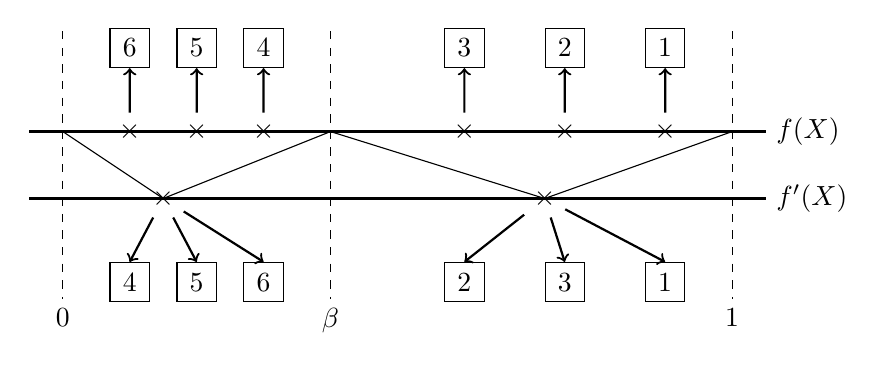
\begin{tikzpicture}[scale=0.85]

\draw[very thick] (-0.5,0.5) -- (10.5,0.5) node[right] {$f(X)$};
\draw[very thick] (-0.5,-0.5) -- (10.5,-0.5) node[right] {$f'(X)$};

\draw[dashed] (0,2) -- (0,-2) node[below] {$0$};
\draw[dashed] (4,2) -- (4,-2) node[below] {$\beta$};
\draw[dashed] (10,2) -- (10,-2) node[below] {$1$};
\draw[] (0, 0.5) -- (1.5, -0.5) {};
\draw[] (4, 0.5) -- (1.5, -0.5) {};
\draw[] (4, 0.5) -- (7.2, -0.5) {};
\draw[] (10, 0.5) -- (7.2, -0.5) {};

\node (x1) at (1, 0.5) {$\times$};
\node (x2) at (2, 0.5) {$\times$};
\node (x3) at (3, 0.5) {$\times$};
\node (x7) at (1.5, -0.5) {$\times$};

\node (x4) at (6, 0.5) {$\times$};
\node (x5) at (7.5, 0.5) {$\times$};
\node (x6) at (9, 0.5) {$\times$};
\node (x8) at (7.2, -0.5) {$\times$};

\node[draw, minimum width=0.5cm, minimum height=0.5cm] (box1) at (1, 1.75) {6};
\node[draw, minimum width=0.5cm, minimum height=0.5cm] (box2) at (2, 1.75) {5};
\node[draw, minimum width=0.5cm, minimum height=0.5cm] (box3) at (3, 1.75) {4};
\node[draw, minimum width=0.5cm, minimum height=0.5cm] (box4) at (6, 1.75) {3};
\node[draw, minimum width=0.5cm, minimum height=0.5cm] (box5) at (7.5, 1.75) {2};
\node[draw, minimum width=0.5cm, minimum height=0.5cm] (box6) at (9, 1.75) {1};

\node[draw, minimum width=0.5cm, minimum height=0.5cm] (box7) at (1, -1.75) {4};
\node[draw, minimum width=0.5cm, minimum height=0.5cm] (box8) at (2, -1.75) {5};
\node[draw, minimum width=0.5cm, minimum height=0.5cm] (box9) at (3, -1.75) {6};
\node[draw, minimum width=0.5cm, minimum height=0.5cm] (box10) at (6, -1.75) {2};
\node[draw, minimum width=0.5cm, minimum height=0.5cm] (box11) at (7.5, -1.75) {3};
\node[draw, minimum width=0.5cm, minimum height=0.5cm] (box12) at (9, -1.75) {1};

\draw[thick, ->] (x1) -- (box1);
\draw[thick, ->] (x2) -- (box2);
\draw[thick, ->] (x3) -- (box3);
\draw[thick, ->] (x4) -- (box4);
\draw[thick, ->] (x5) -- (box5);
\draw[thick, ->] (x6) -- (box6);

\draw[thick, ->] (x7) -- (box8.north);
\draw[thick, ->] (x7) -- (box9.north);
\draw[thick, ->] (x7) -- (box7.north);
\draw[thick, ->] (x8) -- (box10.north);
\draw[thick, ->] (x8) -- (box12.north);
\draw[thick, ->] (x8) -- (box11.north);

\end{tikzpicture}
\caption{Job sequencing under fine-grained (above) and coarse (below) calibrated predictors. For six example jobs, predicted probabilities $p_i$ are marked with $\times$, and numbered boxes give the order of jobs according to each predictor.}
\label{fig: job-seq}
\end{figure}

\paragraph{Performance analysis.} Building off of Equation~\eqref{eq:scheduling_CR}, we bound the expected competitive ratio $\E[\CR(\cA)]$ by bounding each of $\E[L(f(\vec{X}), \vec{Y})]$, $\E[M(f(\vec{X}), \vec{Y})]$, and $\E[N(f(\vec{X}), \vec{Y})]$. The dependence on the ordering of predictions from $f$ in these random counts means our analysis heavily involves functions of order statistics. For example, considering the shared summand of $L(\cdot)$ and $N(\cdot)$,
\begin{align*}
    \E\left[\mathbbm{1}_{\{\vec{Y}_{(i)} = 0 \}}\cdot \mathbbm{1}_{\{\vec{Y}_{(j)} = 1 \}} \mid f(\vec{X}) \right]
    &=  \biggl(\Pr[\vec{Y}_{(i)} = 0 \mid f(\vec{X}_{(i)}) ] \cdot  \Pr[\vec{Y}_{(j)} = 0 \mid f(\vec{X}_{(j)})] \biggr)\\
    &= (1-f(\vec{X}_{(i)}))f(\vec{X}_{(j)})\\
    &= g(f(\vec{X}_{(i)}), f(\vec{X}_{(j)}))
\end{align*}
for the function $g(x,y) = (1-x)y$. Similarly, the analysis for the summand of $M(\cdot)$ yields $g(f(\vec{X}_{(i)}), f(\vec{X}_{(j)}))$ for $g(x,y) = (1-x)(1-y)$. Based on this, our high-level strategy is to relate ``ordered" expectations of the form
\[\E\left[\sum_{i=1}^n \sum_{j=i+1}^n g\bigl(f(\vec{X}_{(i)}), f(\vec{X}_{(j)})\bigr)\right] \]
to their ``unordered" counterparts
\[\E\left[\sum_{i=1}^n \sum_{j=i+1}^n g\bigl(f(\vec{X}_{i}), f(\vec{X}_{j})\bigr),\right] \]
which are simple to compute. \cref{lemma: sym-unorder} shows that the ordered and unordered expectations are, in fact, equivalent when the function $g$ satisfies $g(x,y)=g(y,x)$. 

\begin{restatable}{lemma}{SymUnordering}\label{lemma: sym-unorder}
Let $X_1, \dots, X_n$ be iid random variables with order statistics $X_{(1)} \geq \dots \geq X_{(n)}$. For any symmetric function $g:\mathbb{R} \times \mathbb{R} \to \mathbb{R}$,
\[\sum_{i=1}^n \sum_{j = i+1}^n g(X_{(i)}, X_{(j)}) = \sum_{i=1}^n \sum_{j = i+1}^n g(X_{i}, X_{j}).\]
\end{restatable}

This result is sufficient to compute the expectation of $M(\cdot)$ exactly. For the other counts, the analysis is more technical as $g(x,y)=(1-x)y$ is not symmetric. \cref{lemma: ordering-gap} characterizes the relationship between the ordered and unordered expectations for the function $g(x,y)=(1-x)y$.
\begin{restatable}{lemma}{OrderingImprov}\label{lemma: ordering-gap}
    Let $X_1, \dots, X_n$ be iid samples from a distribution over the unit interval $[0,1]$ with order statistics $X_{(1)} \geq \dots \geq X_{(n)}$. Then,
    \begin{align*}
    \E\left[\sum_{i=1}^n \sum_{j = i+1}^n (1-X_{(i)}) \cdot X_{(j)}\right] \leq \E\left[\sum_{i=1}^n \sum_{j = i+1}^n (1-X_{i}) \cdot X_{j}\right]  &-  \binom{n}{2} \cdot \mathrm{Var}(X_1).
    \end{align*}
\end{restatable}
\begin{proof}[Proof sketch]
    By \cref{lemma: sym-unorder} with $g(x,y)=xy$,
    \[\sum_{i=1}^n \sum_{j = i+1}^n X_{(i)} \cdot X_{(j)} = \sum_{i=1}^n \sum_{j = i+1}^n X_{i} \cdot X_{j}\] can be removed from both sides. Then, we apply \cref{lemma: sym-unorder} with $g(x,y)=\min(x,y)$ to simplify the left-hand-side.
    \begin{align*}
        \sum_{i=1}^n \sum_{j=i+1}^n X_{(j)} &= \sum_{i=1}^n \sum_{j=i+1}^n \min\{X_{(i)}, X_{(j)}\} \\
        &= \sum_{i=1}^n \sum_{j=i+1}^n \min\{X_i, X_j\}.
    \end{align*}
    Finally, we show that $\E[X_1 - \min\{X_1, X_2\}] \geq \mathrm{Var}(X_1)$. Note that $\E[X_1] - \E[\min\{X_1, X_2\}] = \frac{1}{2} \E |X_1-X_2|$ since
    \[X_1 - \min\{X_1, X_2\} = \begin{cases} 
    0 &\text{if $X_1 \leq X_2$}\\
    |X_1-X_2| &\text{if $X_1 > X_2$}.\end{cases}\]
    Finally, $\E|X_1-X_2| \geq \E|X_1 - X_2|^2 = 2\mathrm{Var}(X_1)$.
\end{proof}
With careful conditioning to deal with random summation bounds, we apply \cref{lemma: ordering-gap} to bound the expectations of $L(\cdot)$ and $N(\cdot)$, giving this section's main theorem. Of note, \cref{thm: schedule-improv} says that the expected number of inversions of high and low priority jobs decreases with predictor granularity, measured by $\kappa_1$ and $\kappa_2$. For the method from \citet{Cho22:Scheduling}, $\kappa_1=\kappa_2=0$ and the inequalities are tight.
\begin{restatable}{theorem}{SchedulingImprov} \label{thm: schedule-improv}
    Let $f$ be calibrated, with $\Pr[f(X) > \beta \mid Y=0]=\epsilon_0$, $\Pr[f(X) \leq \beta \mid Y=1]=\epsilon_1$,     \begin{align*}
        \kappa_1 &= \Pr[f(X) > \beta]^2 \cdot \mathrm{Var}(f(X) \mid f(X) > \beta) \text{, and} \\
        \kappa_2 &= \Pr[f(X) \leq \beta]^2 \cdot \mathrm{Var}(f(X) \mid f(X) \leq \beta).
    \end{align*} 
    Then
    \vspace{-3mm}
    \begin{enumerate}
        \itemsep0em 
        \item $\E[L(f(\vec{X}), \vec{Y})] \leq \binom{n}{2}\bigl(\rho(1-\rho)(1+\epsilon_0)\epsilon_1 - \kappa_1\bigr)$
        \item $\E[M(f(\vec{X}), \vec{Y})] = \binom{n}{2}(1-\rho)^2 \epsilon_0^2$
        \item $\E[N(f(\vec{X}), \vec{Y})] \leq \binom{n}{2}\bigl(\rho(1-\rho)\epsilon_0(1-\epsilon_1) - \kappa_2\bigr)$
    \end{enumerate}
\end{restatable}
\begin{remark}
    $\cA$ is 1-consistent: $\ALG(\cA, \; \cdot) -\OPT(\cdot) = 0$ when $\epsilon_0 = \epsilon_1 = 0$.
\end{remark}
\section{Experiments}
\label{sec: experiments}

\begin{table*}
        % \centering
        \caption{A comparison between our proposed method with other advanced methods on the nuScenes test set.
        % This leaderboard is available at \href{https://www.nuscenes.org/tracking?externalData=all&mapData=all&modalities=Any}{nuScenes official benchmark}.
        $\ddagger$ means the GPU device.
        \textcolor{black}{The reported runtimes of all methods exclude the detection time.}
        Poly-MOT~\cite{li2023poly}, Fast-Poly~\cite{li2024fast} and Easy-Poly rely entirely on the detector input, as they do not utilize any visual or deep features \textcolor{black}{during tracking}.}
        \label{table:nu_test}
        % \renewcommand{\arraystretch}{0.7}
        \setlength{\tabcolsep}{1.6mm}
        {
        \begin{tabular}{cccc|ccc|ccc}
        \toprule
        \multicolumn{1}{c}{\textbf{Method}} & \textbf{Device} & \textbf{Detector} & \textbf{Input} & \textbf{AMOTA}$\uparrow$ & \textbf{MOTA}$\uparrow$ & \textbf{FPS}$\uparrow$ & \textbf{IDS}$\downarrow$ & \textbf{FN}$\downarrow$ & \textbf{FP}$\downarrow$ \\ \midrule
                                     EagerMOT~\cite{kim2021eagermot}               & \textbf{\text{--}}       & CenterPoint~\cite{yin2021center}\&Cascade R-CNN~\cite{cai2018cascade}         & 2D+3D       & 67.7      & 56.8     & 4    & 1156    & 24925   & 17705   \\
                                   CBMOT~\cite{benbarka2021score}     & I7-9700          & CenterPoint~\cite{yin2021center}\&CenterTrack~\cite{zhou2020tracking}          & 2D+3D         & 67.6      & 53.9      & \textcolor{red}{80.5}    & 709    & 22828   & 21604   \\
                                   % ShaSTA~\cite{sadjadpour2023shasta} & A100$\ddagger$       & CenterPoint~\cite{yin2021center}         & 3D      & 69.6      & 57.8     & 10     & 473    & 21293   & 16746   \\
                                   Minkowski~\cite{gwak2022minkowski} & TITAN$\ddagger$  & Minkowski~\cite{gwak2022minkowski}         & 3D      & 69.8      & 57.8     & 3.5    & 325    & 21200   & 19340   \\
                                   ByteTrackv2~\cite{zhang2023bytetrackv2} & \textbf{\text{--}}       & TransFusion-L~\cite{bai2022transfusion}         & 3D      & 70.1      & 58     & \textbf{\text{--}}    & 488    & 21836   & 18682   \\
                                   3DMOTFormer~\cite{ding20233dmotformer}& 2080Ti$\ddagger$       & BEVFuison~\cite{liu2023bevfusion}       & 2D+3D      & 72.5      & 60.9     & \textcolor{blue}{54.7}    & 593    & 20996   & \textcolor{blue}{17530}   \\  
                                   %CAMO-MOT~\cite{li2023camo}& 3090Ti$\ddagger$   & BEVFuison~\cite{liu2023bevfusion}\&FocalsConv~\cite{chen2022focal}   & 2D+3D      & 75.3      & \textbf{63.5}     & \textbf{\text{--}}    & 324    & 18192   & 17269   \\
                                   Poly-MOT~\cite{li2023poly}               & 9940X       & LargeKernel3D~\cite{chen2022scaling}         &2D+3D       & \textcolor{blue}{75.4}      & \textcolor{blue}{62.1}     & 3    & \textcolor{blue}{292}    & \textcolor{blue}{17956}   & 19673   \\ 
                                  Fast-Poly~\cite{li2024fast}               & 7945HX       & LargeKernel3D~\cite{chen2022scaling}         &2D+3D       & \textcolor{blue}{75.8}      & \textcolor{blue}{62.8}     & 34.2    & \textcolor{blue}{326}    & \textcolor{blue}{18415}   &  \textcolor{blue}{17098}  \\ \midrule

                                  \textbf{Easy-Poly (Ours)}               & 4090Ti$\ddagger$       & LargeKernel3D~\cite{chen2022scaling}         &2D+3D       &  \textcolor{red}{75.9}      & \textcolor{red}{63.0}     & \textcolor{blue}{34.9}    & \textcolor{red}{287}    & \textcolor{red}{17620}   &   \textcolor{red}{16718}  \\
        \bottomrule
        \end{tabular}}
        % \vspace{-1.5em}
 \end{table*}


\begin{table*}
\vspace{0.5em}
\begin{center}
\caption{
{A comparison of existing methods applied to the nuScenes val set.}}
\label{table:nu_val}
% \renewcommand{\arraystretch}{0.7}
\setlength{\tabcolsep}{2.4mm}
{
\begin{tabular}{cccccccc}
\toprule
\bf{Method} & \bf{Detector} & \bf{Input Data} & \bf{MOTA$\uparrow$} & \bf{AMOTA$\uparrow$} & \bf{AMOTP$\downarrow$} & \bf{FPS$\uparrow$} & \bf{IDS$\downarrow$}  \\ \hline
CBMOT~\cite{benbarka2021score}   & CenterPoint~\cite{yin2021center} \& CenterTrack~\cite{zhou2020tracking} & 2D + 3D & -- & 72.0 & \textbf{\textcolor{red}{48.7}}  & -- & 479   \\
EagerMOT~\cite{kim2021eagermot}  & CenterPoint~\cite{yin2021center} \& Cascade R-CNN~\cite{cai2018cascade} & 2D + 3D  & -- & 71.2   & 56.9 & 13  & 899    \\
SimpleTrack~\cite{pang2022simpletrack}  & CenterPoint~\cite{yin2021center} & 3D & 60.2 & 69.6  & 54.7 & 0.5  & 405  \\
CenterPoint~\cite{yin2021center}   & CenterPoint~\cite{yin2021center} & 3D & -- & 66.5  & 56.7 & -- & 562 \\ 
OGR3MOT~\cite{zaech2022learnable}  & CenterPoint~\cite{yin2021center} &3D & 60.2 & 69.3  & 62.7 & 12.3 & \textbf{\textcolor{blue}{262}}  \\ \hline

\textbf{Poly-MOT}~\cite{li2023poly}      & CenterPoint~\cite{yin2021center} & 3D & 61.9 & 73.1   & \textbf{\textcolor{blue}{52.1}} & 5.6 & 281   \\ 
% \textbf{Poly-MOT}~\cite{li2023poly}      & LargeKernel3D-L~\cite{chen2022scaling}  & 3D   & \textbf{\textcolor{red}{75.2}}    & 54.1   & \textbf{\textcolor{red}{252}} \\ 

\textbf{Poly-MOT}~\cite{li2023poly}      & LargeKernel3D-L~\cite{chen2022scaling}  & 3D & 54.1 & \textbf{\textcolor{red}{75.2}}    & 54.1  & 8.6 & 252 \\

\textbf{Fast-Poly}~\cite{li2024fast}      & CenterPoint~\cite{yin2021center} & 3D & \textbf{\textcolor{blue}{63.2}}  & 73.7   &  -- & \textbf{\textcolor{blue}{28.9}} & 414   \\ \hline
 
\textbf{Easy-Poly (Ours)}       & CenterPoint~\cite{yin2021center} & 2D + 3D & \textbf{\textcolor{blue}{64.4}} & \textbf{\textcolor{blue}{74.5}}   & 54.9  & \textbf{\textcolor{blue}{34.6}} & \textbf{\textcolor{blue}{272}}   \\
\textbf{Easy-Poly (Ours)}       & LargeKernel3D~\cite{chen2022scaling}  & 2D + 3D  & \textbf{\textcolor{red}{64.8}} & \textbf{\textcolor{blue}{75.0}}    & \textbf{\textcolor{blue}{53.6}}  & \textbf{\textcolor{red}{34.9}}  & \textbf{\textcolor{red}{242}} \\ \hline
% \vspace{-4.5em}
% \setlength{\abovecaptionskip}{3pt}
% \setlength{\belowcaptionskip}{3pt}
\end{tabular}}
\end{center}
\end{table*}

\subsection{Datasets}

% The nuScenes dataset~\cite{caesar2020nuscenes} consists of 850 training and 150 test sequences, capturing a wide range of driving scenarios, including challenging weather conditions and nighttime environments. Each sequence contains approximately 40 frames, with keyframes sampled at 2Hz and fully annotated. In addition to this, it provides annotations for object-level attributes such as visibility, activity, pose, and more. It includes a large volume of RGB and point-cloud data (in PCD format). The official evaluation protocol utilizes \textbf{AMOTA}, \textbf{MOTA}, and \textbf{sAMOTA}~\cite{weng20203d} as primary metrics, evaluating performance across seven object categories: Car (\textit{Car}), Bicycle (\textit{Bic}), Motorcycle (\textit{Moto}), Pedestrian (\textit{Ped}), Bus (\textit{Bus}), Trailer (\textit{Tra}), and Truck (\textit{Tru}). Given the substantial size of the complete nuScenes dataset, users often prefer the nuScenes-mini dataset. Notably, Poly-MOT, Fast-Poly, and our proposed Easy-Poly methods exclusively utilize keyframes for tracking tasks.


The nuScenes dataset~\cite{caesar2020nuscenes} consists of 850 training and 150 test sequences, capturing a wide range of driving scenarios, including challenging weather conditions and nighttime environments. Each sequence contains approximately 40 frames, with keyframes sampled at 2Hz and fully annotated. The official evaluation protocol utilizes \textbf{AMOTA}, \textbf{MOTA}, and \textbf{sAMOTA}~\cite{weng20203d} as primary metrics, evaluating performance across seven object categories: Car (\textit{Car}), Bicycle (\textit{Bic}), Motorcycle (\textit{Moto}), Pedestrian (\textit{Ped}), Bus (\textit{Bus}), Trailer (\textit{Tra}), and Truck (\textit{Tru}). Notably, Poly-MOT, Fast-Poly, and our proposed Easy-Poly methods exclusively utilize keyframes for tracking tasks.

\subsection{Implementation Details}

% Our tracking method is implemented in Python under the Nvidia 4090X GPU.  Hyperparameters are chosen based on the best AMOTA identified in the validation set. SF thresholds are category-specific and detector-specific, which are (\textit{Bic}: 0.15; are (\textit{Car}: 0.16; are (\textit{Moto}: 0.16; \textit{Bus}: 0.12; \textit{Tra}: 0.13; \textit{Tru}: 0; \textit{Ped}: 0.13) on nuScenes on Waymo. The NMS thresholds are 0.08 on all categories and datasets. We also employ Scale-NMS~\cite{huang2021bevdet} on (\textit{Bic}, \textit{Ped}) on nuScenes. With default $IoU_{bev}$ in NMS, we additionally utilize our proposed $A\text{-}gIoU_{bev}$ to describe similarity for (\textit{Bic}, \textit{Ped}, \textit{Bus}, \textit{Tru}) on nuScenes. The motion models and filters are consistent with~\cite{li2023poly}. The lightweight filter is implemented by the median filter with $l_{lw}=5$ on all datasets. The association metrics are all implemented by $A\text{-}gIoU$ on all datasets. The first association thresholds $\theta_{fm}$ are category-specific, which are (\textit{Bic, Moto, Bus}: 1.6; \textit{Car, Tru}: 1.2; \textit{Tra}: 1.16;\textit{Ped}: 1.78) on nuScenes. Voxel mask size $\theta_{vm}$ is 5\textit{m} on nuScenes.  The count-based and output file strategies are consistent with~\cite{li2023poly}. In the confidence-based part, decay rates $\sigma$ are category-specific, which are (\textit{Ped}: 0.18; \textit{Car}: 0.26; \textit{Tru, Moto}: 0.28; \textit{Tra}: 0.22; \textit{Bic,Bus}: 0.24) on nuScenes. The delete threshold $\theta_{dl}$ are (\textit{Bus}: 0.08,  \textit{Ped}: 0.1 and 0.04 for other categories) on nuScenes.

Our tracking framework is implemented in Python and executed on an Nvidia 4090X GPU. Hyperparameters are optimized based on the highest AMOTA achieved on the validation set. The following category-specific and SF thresholds are employed for nuScenes: (\textit{Bic}: 0.15; \textit{Car}: 0.16; \textit{Moto}: 0.16; \textit{Bus}: 0.12; \textit{Tra}: 0.13; \textit{Tru}: 0; \textit{Ped}: 0.13). NMS thresholds are uniformly set to 0.08 across all categories and datasets. Additionally, we implement Scale-NMS~\cite{huang2021bevdet} for (\textit{Bic}, \textit{Ped}) categories on nuScenes.
In conjunction with the default in NMS, we introduce our novel  metric to enhance similarity assessment for (\textit{Bic}, \textit{Ped}, \textit{Bus}, \textit{Tru}) categories on nuScenes. Motion models and filters are consistent with those described in~\cite{li2023poly}. A lightweight filter, implemented as a median filter with , is applied across all datasets. Association metrics universally employ  across all datasets.
Category-specific first association thresholds  for nuScenes are as follows: (\textit{Bic, Moto, Bus}: 1.6; \textit{Car, Tru}: 1.2; \textit{Tra}: 1.16; \textit{Ped}: 1.78). The voxel mask size  is set to 5\textit{m} on nuScenes. Count-based and output file strategies align with those presented in~\cite{li2023poly}.
In the confidence-based component, category-specific decay rates for nuScenes are: (\textit{Ped}: 0.18; \textit{Car}: 0.26; \textit{Tru, Moto}: 0.28; \textit{Tra}: 0.22; \textit{Bic, Bus}: 0.24). The delete thresholds  are set as follows: (\textit{Bus}: 0.08, \textit{Ped}: 0.1, and 0.04 for all other categories) on nuScenes.

In the object tracking phase of 3D MOT, Easy-Poly exhibits exceptional performance following a series of optimizations. These enhancements include pre-processing, Kalman filtering, motion modeling, and tracking cycle refinements. The integration of these techniques significantly improves the algorithm's effectiveness in complex 3D environments.

Easy-Poly exhibits exceptional performance on the test set, achieving a \textbf{75.9\%} AMOTA score, surpassing the majority of existing 3D MOT methods. As shown in Table \ref{table:nu_test}, Easy-Poly attains a remarkably low IDS count of \textbf{287} while maintaining the highest AMOTA (\textbf{75.9\%}) among all modal methods. This underscores Easy-Poly's ability to maintain stable tracking without compromising recall. Notably, Easy-Poly achieves state-of-the-art performance without relying on additional image data input. Easy-Poly significantly outperforms competing algorithms in the critical 'Car' category. With minimal computational overhead, it delivers impressive results, highlighting its potential for integration into real-world autonomous driving systems. The False Negative and False Positive metrics in Table \ref{table:nu_test} further demonstrate Easy-Poly's robust continuous tracking capability while maintaining high recall.

For validation set experiments in Table \ref{table:nu_val}, we utilize CenterPoint~\cite{yin2021center} as the detector to ensure fair comparisons. As illustrated in Table \ref{table:nu_val}, Easy-Poly significantly outperforms most deep learning-based methods in both tracking accuracy (\textbf{75.0\%} AMOTA, \textbf{64.8\%} MOTA) and computational efficiency (\textbf{34.9} FPS). Compared to the baseline FastPoly~\cite{li2024fast}, Easy-Poly achieves substantial improvements of \textbf{+1.3\%} in MOTA and \textbf{+1.6\%} in AMOTA, while operating \textbf{1.5x} faster under identical conditions. When integrated with the high-performance LargeKernel3D~\cite{chen2022scaling} detector, Easy-Poly demonstrates even more impressive detection and tracking capabilities. Furthermore, when employing the multi-camera detector \textcolor{black}{DETR3D}~\cite{DETR3D} with constrained performance, Easy-Poly exhibits robust real-time performance without compromising accuracy. Furthermore, the lower AMOTP and IDS metrics demonstrate Easy-Poly's exceptional capability in tracking small objects and maintaining performance in complex scenarios and adverse weather conditions. These results underscore the algorithm's robustness across diverse and challenging environments.
% It is noteworthy that achieving optimal AMOTA necessitates a stringent score filter threshold, which marginally reduces the latency advantage of our method. Nevertheless, Easy-Poly maintains a favorable balance between accuracy and computational efficiency.

\begin{table}
% \vspace{0.5em}
        \caption{Comparing different data association algorithms using CenterPoint and (lines 1-7) and LargeKernel3D (lines 8-11) methods on nuScenes val set. Among them, the algorithms lines 1-3 are the Fast-Poly framework and in lines 4-11 are the latest our Easy-Poly framework.}

        \label{table:nus_assoc}
        % \renewcommand{\arraystretch}{0.7}
        \setlength{\tabcolsep}{0.1mm}
        \begin{tabular}{cccccc}
        \toprule
        \multicolumn{1}{c}{\textbf{Algorithms}} & \textbf{MOTA}$\uparrow$ & \textbf{AMOTA}$\uparrow$ & \textbf{AMOTP}$\downarrow$ & \textbf{IDS}$\downarrow$ & \textbf{FN}$\downarrow$\\ 
        
        \midrule
         %  Mutual Nearest Neighbor (MNN)
         MNN  & 62.2  & 72.5 & 52.4  & 433 & 16644  \\  
         Greedy    & 62.3  & 72.7 &  53.4  & 428  & 17647 \\
         Hungarian & \textbf{\textcolor{blue}{63.2}}  & \textbf{\textcolor{blue}{73.7}} & \textbf{\textcolor{blue}{52.1}} & \textbf{\textcolor{blue}{414}}  & \textbf{\textcolor{blue}{15996}}  \\
        
        \midrule  
        % 多模态+数据增强
         %  Mutual Nearest Neighbor (MNN)
        \textbf{MNN (Ours)}  & 63.7  & 73.6 & 54.8  & 406 &  \textbf{\textcolor{red}{15873 }}\\  
        \textbf{Greedy (Ours)}    &  64.0  & 73.7  &  54.6  & 368  & 16736 \\
        \textbf{Hungarian (Ours)}  & 64.3  & 74.3 & \textbf{\textcolor{red}{54.3}} &  335 & 16892  \\

        \textbf{DTO (Ours)}   & \textbf{\textcolor{red}{64.4}}  &   \textbf{\textcolor{red}{74.5}} & 54.9 &  \textbf{\textcolor{red}{272}} & 16982  \\

        
         \midrule
         \textbf{MNN (Ours)}  & 64.1  & 73.9 & 54.0  & 370 & 15865  \\  
         \textbf{Greedy (Ours)}    & 64.5  & 74.3 & 53.7  & 307  & 16014 \\
        \textbf{Hungarian (Ours)}  & 64.7  & 74.8 & 53.9  & 291  & 15923 \\

        \textbf{DTO (Ours)}  & \textbf{\textcolor{red}{64.8}}  & \textbf{\textcolor{red}{75.0}} & \textbf{\textcolor{red}{53.6}}  & \textbf{\textcolor{red}{242}}  & \textbf{\textcolor{red}{15488}} \\

    \bottomrule
\end{tabular}
\end{table}



% \begin{table}
% \caption{The ablation study of whether or not to use Score Filter and Non-Maximum Suppression, including the Run-Time, which represents the execution time of the Pre-processing Module. We compared Poly-MOT~\cite{li2023poly} (rows 1-3) with our proposed Easy-Poly method (rows 4-6).}
% \label{table:nu_NMSsf}
% % \renewcommand{\arraystretch}{0.7}
% \setlength{\tabcolsep}{2.7mm}
% {
% \begin{tabular}{cccc}
% \toprule

% \textbf{Variable} & \textbf{AMOTA$\uparrow$} & \textbf{IDS$\downarrow$} &
% \textbf{Run-Time (s) $\downarrow$}
% \\ 
% \midrule
% NMS + SF & \textbf{\textcolor{blue}{73.1}}   & \textbf{\textcolor{blue}{281}}  & 0.055    \\
% NMS     & 71.8  & 320  & 0.093     \\
% SF       & 68.6  & 354  & \textbf{\textcolor{blue}{0.008}}     \\ 
% \midrule
% \textbf{NMS + SF (Ours)} & \textbf{\textcolor{red}{75.0}}   & \textbf{\textcolor{red}{242}}  & 0.037    \\
% \textbf{NMS (Ours)}      & 73.6   & 273  & 0.068    \\
% \textbf{SF (Ours)}       & 71.2   & 308  & \textbf{\textcolor{red}{0.008}}     \\\hline
% % \vspace{-3.2em}
% \end{tabular}}
% \end{table}



\subsection{Comparative Evaluations} 
\label{sec: Comparative}

% Our proposed method, Easy-Poly, achieves state-of-the-art performance on the nuScenes validation set, demonstrating \textbf{75.0\%} AMOTA at \textbf{34.9} FPS, surpassing existing approaches. Utilizing an identical detector, Easy-Poly outperforms Fast-Poly \cite{li2024fast} across nearly all key metrics, with notable improvements in accuracy (\textbf{+1.3\%} AMOTA, \textbf{+1.6\%} MOTA) and speed (\textbf{+6.0 FPS}). While marginally slower than CBMOT \cite{benbarka2021score} and 3DMOTFormer \cite{ding20233dmotformer}, Easy-Poly significantly exceeds their accuracy while maintaining robust real-time performance. Our open-source implementation establishes a strong baseline for 3D MOT, providing a solid foundation for future advancements in the field.

In this study, we conduct a comprehensive evaluation of the association stage, focusing on four algorithms: Hungarian, Greedy, MNN, and the novel DTO. Our extensive experiments, summarized in Table~\ref{table:nus_assoc}, reveal that the Easy-Poly consistently outperforms Fast-Poly across both CenterPoint and LargeKernel3D frameworks. Notably, LargeKernel3D demonstrates superior performance over CenterPoint, particularly in complex tracking scenarios. Among the association algorithms, Hungarian and DTO consistently yield superior results, underscoring their robustness and efficacy in diverse multi-object tracking contexts. Compared to the Hungarian algorithm, DTO not only achieves similarly excellent AMOTA values but also provides more robust and accurate tracking performance, especially in challenging scenarios involving occlusions, missed detections, or false positives. These findings highlight the critical role of algorithm selection and model optimization in advancing the state-of-the-art in 3D object tracking.

\begin{figure*}[t]
    \centering
    \includegraphics[width=0.95\linewidth]{Images/Ablation_study_line_chart_for_NMS.pdf}
    \vspace{-8pt}
    \caption
    {
      The ablation study of whether or not to use Score Filter and Non-Maximum Suppression, including the Run-Time, which represents the execution time of the Pre-processing Module. We compared Poly-MOT with our proposed Easy-Poly method.
     }
     \Description{}
    \label{fig: NMSFS}
\end{figure*}


\textcolor{black}{Table \ref{table:nu_life} demonstrates the efficacy of our proposed methods. The Fast-Poly tracklet termination strategy (line 3) significantly outperforms baseline score refinement~\cite{benbarka2021score} (line 2), yielding a \textbf{2.7\%} improvement in AMOTA and reducing FN by \textbf{2366}. This enhancement mitigates tracker vulnerabilities in mismatch scenarios, including occlusions. Further performance gains are achieved through smoother score prediction (line 4), resulting in additional improvements of \textbf{0.4\%} AMOTA, \textbf{0.1\%} MOTA, and a reduction of \textbf{926 FN}.}
Our Easy-Poly model exhibits even more substantial performance enhancements. The tracklet termination strategy (line 7) surpasses the baseline score refinement (line 6) by \textbf{2.8\%} in AMOTA while decreasing FN by \textbf{1844}. Furthermore, the integration of smoother score prediction (line 8) further boosts the tracking performance, resulting in improvements of \textbf{0.4\%} in AMOTA and \textbf{0.6\%} in MOTA, along with a reduction of \textbf{575} FN.


\begin{table}
% \vspace{0.5em}
        \caption{A comparison on distinct life-cycle modules on nuScenes val set.
        \textbf{Average} means using the online average score to delete.
        \textbf{Latest} means using the latest score to delete.
        \textbf{Max-age} means using the continuous mismatch time to delete.
        Other settings are under the best performance. Methods in lines 1-4 and lines 5-8 use Fast-Poly~\cite{li2024fast} and Our Easy-Poly.
        }
        \label{table:nu_life}
        % \renewcommand{\arraystretch}{0.7}
        \setlength{\tabcolsep}{0.1mm}
        \begin{tabular}{ccccc}
        \toprule
        \multicolumn{1}{c}{\textbf{Strategy}} & \textbf{AMOTA}$\uparrow$ & \textbf{MOTA}$\uparrow$ & \textbf{FPS}$\uparrow$ & \textbf{FN}$\downarrow$\\ \midrule
 
         Count                \& Max-age            & 73.3      & 62.9     & 23.0  & 16523    \\
         %predict:normal update:normal+delete = -100
         Confidence~\cite{benbarka2021score} \& Latest       & 70.6      & 63.2     & \textbf{\textcolor{blue}{45.8}}  & 19192   \\%predict:minus update:multi+latest
         Confidence~\cite{benbarka2021score} \& Average      & 73.3      & 63.1     & 28.3 & 16826   \\%predict:minus update:multi+average
         Confidence  \& Average      & \textbf{\textcolor{blue}{73.7}}      & \textbf{\textcolor{blue}{63.2}}     & 28.9  & \textbf{\textcolor{blue}{15900}}   \\%predict:normal update:multi+average 27.7or28.9
         \midrule
         \textbf{Count \& Max-age (Ours)}          & 74.3      & 63.8     & 34.3  & 16024    \\
         %predict:normal update:normal+delete = -100
         \textbf{Confidence~\cite{benbarka2021score} \& Latest (Ours)}        & 71.8      & 63.7     & \textbf{\textcolor{red}{50.2}}  & 17907   \\%predict:minus update:multi+latest
         \textbf{Confidence~\cite{benbarka2021score} \& Average (Ours)}       & 74.6      & 64.2     & 35.6 & 16063   \\%predict:minus update:multi+average
         \textbf{Confidence \& Average (Ours)}      & \textbf{\textcolor{red}{75.0}}      & \textbf{\textcolor{red}{64.8}}     & 36.9  & \textbf{\textcolor{red}{15488}}   \\%predict:normal update:multi+average 36.9
        \bottomrule
        \end{tabular}
    \end{table}


\subsection{Ablation Studies}

% The Sf can filter out low-score bounding boxes while NMS can remove duplicate bounding boxes with high confidence, which makes the remaining bounding boxes have superior quality. For the Poly-MOT, using SF before NMS brings inference 40\% reduction in pre-processing inference time while boosting AMOTA by 1.3\% compared with only using NMS. The Fast-Poly has better performance, using SF before NMS brings inference 50\% reduction in pre-processing inference time while boosting AMOTA by 1.4\% compared with only using NMS, as demonstrate in Table~\ref{table:nu_NMSsf}.  It is clear from the table that when only SF is used without NMS, although the running time is fast, both AMOTA and IDS values become lower and the values drop very significantly.

We optimize two-stage filtering approach that synergistically combines SF and NMS to significantly enhance bounding box quality in multi-object tracking scenarios. This novel method effectively integrates SF to eliminate low-score detections and NMS to remove high-confidence duplicates, resulting in a set of superior quality bounding boxes. Our comprehensive experimental results, presented in Figure~\ref{fig: NMSFS}, demonstrate substantial improvements in both computational efficiency and tracking accuracy across multiple state-of-the-art models. For the Poly-MOT model, our approach of applying SF before NMS yields a remarkable \textbf{40\%} reduction in pre-processing inference time while simultaneously improving AMOTA by \textbf{1.3\%} compared to using NMS alone. These results highlight the significant potential of our method in improving real-time tracking capabilities without compromising accuracy. The Easy-Poly model exhibits even more impressive performance gains, further validating the scalability and effectiveness of our approach. By applying SF before NMS, we achieve a substantial \textbf{50\%} reduction in pre-processing time coupled with a \textbf{1.4\%} improvement in AMOTA. This notable improve in both speed and accuracy underscores the robustness of our method across different model architectures. Importantly, our analysis reveals critical insight into the interplay between SF and NMS. Although using SF without NMS accelerates processing, it leads to significant degradation in both AMOTA and Identity Switches IDS metrics. This observation underscores the crucial importance of our combined SF-NMS approach in maintaining an optimal balance between processing speed and tracking accuracy. The synergistic effect of SF and NMS not only enhances the quality of bounding boxes but also optimizes the trade-off between computational efficiency and tracking performance. This balance is particularly vital in real-world applications where both speed and accuracy are paramount, such as autonomous driving and surveillance systems. 
% The consistent improvements observed across different models suggest broad applicability and potential for integration into various tracking frameworks, paving the way for more efficient and accurate tracking systems in complex, real-world environments.


% \subsection{Visualization}

\section{Conclusion}
In this study, we introduce \ours, a novel framework designed to achieve lossless acceleration in generating ultra-long sequences with \acp{llm}. By analyzing and addressing three challenges, \ours significantly enhances the efficiency of the generation process. Our experimental results demonstrate that \ours achieves over $3\times$ acceleration across various model scales and architectures. Furthermore, \ours effectively mitigates issues related to repetitive content, ensuring the quality and coherence of the generated sequences. These advancements position \ours as a scalable and effective solution for ultra-long sequence generation tasks.

\section*{Acknowledgements}
Judy Hanwen Shen is supported by the Simons Foundation Collaboration on the Theory of Algorithmic Fairness, Anders Wikum is supported by a National Defense Science \& Engineering Graduate (NDSEG) fellowship, and Ellen Vitercik acknowledges the support of NSF grant CCF-2338226. We thank Bailey Flanigan for stimulating early discussions that inspired us to pursue this research direction, and Ziv Scully for a technical insight in the proof of \cref{lemma: ordering-gap}.
\endgroup

\bibliography{references}
\subsection{Lloyd-Max Algorithm}
\label{subsec:Lloyd-Max}
For a given quantization bitwidth $B$ and an operand $\bm{X}$, the Lloyd-Max algorithm finds $2^B$ quantization levels $\{\hat{x}_i\}_{i=1}^{2^B}$ such that quantizing $\bm{X}$ by rounding each scalar in $\bm{X}$ to the nearest quantization level minimizes the quantization MSE. 

The algorithm starts with an initial guess of quantization levels and then iteratively computes quantization thresholds $\{\tau_i\}_{i=1}^{2^B-1}$ and updates quantization levels $\{\hat{x}_i\}_{i=1}^{2^B}$. Specifically, at iteration $n$, thresholds are set to the midpoints of the previous iteration's levels:
\begin{align*}
    \tau_i^{(n)}=\frac{\hat{x}_i^{(n-1)}+\hat{x}_{i+1}^{(n-1)}}2 \text{ for } i=1\ldots 2^B-1
\end{align*}
Subsequently, the quantization levels are re-computed as conditional means of the data regions defined by the new thresholds:
\begin{align*}
    \hat{x}_i^{(n)}=\mathbb{E}\left[ \bm{X} \big| \bm{X}\in [\tau_{i-1}^{(n)},\tau_i^{(n)}] \right] \text{ for } i=1\ldots 2^B
\end{align*}
where to satisfy boundary conditions we have $\tau_0=-\infty$ and $\tau_{2^B}=\infty$. The algorithm iterates the above steps until convergence.

Figure \ref{fig:lm_quant} compares the quantization levels of a $7$-bit floating point (E3M3) quantizer (left) to a $7$-bit Lloyd-Max quantizer (right) when quantizing a layer of weights from the GPT3-126M model at a per-tensor granularity. As shown, the Lloyd-Max quantizer achieves substantially lower quantization MSE. Further, Table \ref{tab:FP7_vs_LM7} shows the superior perplexity achieved by Lloyd-Max quantizers for bitwidths of $7$, $6$ and $5$. The difference between the quantizers is clear at 5 bits, where per-tensor FP quantization incurs a drastic and unacceptable increase in perplexity, while Lloyd-Max quantization incurs a much smaller increase. Nevertheless, we note that even the optimal Lloyd-Max quantizer incurs a notable ($\sim 1.5$) increase in perplexity due to the coarse granularity of quantization. 

\begin{figure}[h]
  \centering
  \includegraphics[width=0.7\linewidth]{sections/figures/LM7_FP7.pdf}
  \caption{\small Quantization levels and the corresponding quantization MSE of Floating Point (left) vs Lloyd-Max (right) Quantizers for a layer of weights in the GPT3-126M model.}
  \label{fig:lm_quant}
\end{figure}

\begin{table}[h]\scriptsize
\begin{center}
\caption{\label{tab:FP7_vs_LM7} \small Comparing perplexity (lower is better) achieved by floating point quantizers and Lloyd-Max quantizers on a GPT3-126M model for the Wikitext-103 dataset.}
\begin{tabular}{c|cc|c}
\hline
 \multirow{2}{*}{\textbf{Bitwidth}} & \multicolumn{2}{|c|}{\textbf{Floating-Point Quantizer}} & \textbf{Lloyd-Max Quantizer} \\
 & Best Format & Wikitext-103 Perplexity & Wikitext-103 Perplexity \\
\hline
7 & E3M3 & 18.32 & 18.27 \\
6 & E3M2 & 19.07 & 18.51 \\
5 & E4M0 & 43.89 & 19.71 \\
\hline
\end{tabular}
\end{center}
\end{table}

\subsection{Proof of Local Optimality of LO-BCQ}
\label{subsec:lobcq_opt_proof}
For a given block $\bm{b}_j$, the quantization MSE during LO-BCQ can be empirically evaluated as $\frac{1}{L_b}\lVert \bm{b}_j- \bm{\hat{b}}_j\rVert^2_2$ where $\bm{\hat{b}}_j$ is computed from equation (\ref{eq:clustered_quantization_definition}) as $C_{f(\bm{b}_j)}(\bm{b}_j)$. Further, for a given block cluster $\mathcal{B}_i$, we compute the quantization MSE as $\frac{1}{|\mathcal{B}_{i}|}\sum_{\bm{b} \in \mathcal{B}_{i}} \frac{1}{L_b}\lVert \bm{b}- C_i^{(n)}(\bm{b})\rVert^2_2$. Therefore, at the end of iteration $n$, we evaluate the overall quantization MSE $J^{(n)}$ for a given operand $\bm{X}$ composed of $N_c$ block clusters as:
\begin{align*}
    \label{eq:mse_iter_n}
    J^{(n)} = \frac{1}{N_c} \sum_{i=1}^{N_c} \frac{1}{|\mathcal{B}_{i}^{(n)}|}\sum_{\bm{v} \in \mathcal{B}_{i}^{(n)}} \frac{1}{L_b}\lVert \bm{b}- B_i^{(n)}(\bm{b})\rVert^2_2
\end{align*}

At the end of iteration $n$, the codebooks are updated from $\mathcal{C}^{(n-1)}$ to $\mathcal{C}^{(n)}$. However, the mapping of a given vector $\bm{b}_j$ to quantizers $\mathcal{C}^{(n)}$ remains as  $f^{(n)}(\bm{b}_j)$. At the next iteration, during the vector clustering step, $f^{(n+1)}(\bm{b}_j)$ finds new mapping of $\bm{b}_j$ to updated codebooks $\mathcal{C}^{(n)}$ such that the quantization MSE over the candidate codebooks is minimized. Therefore, we obtain the following result for $\bm{b}_j$:
\begin{align*}
\frac{1}{L_b}\lVert \bm{b}_j - C_{f^{(n+1)}(\bm{b}_j)}^{(n)}(\bm{b}_j)\rVert^2_2 \le \frac{1}{L_b}\lVert \bm{b}_j - C_{f^{(n)}(\bm{b}_j)}^{(n)}(\bm{b}_j)\rVert^2_2
\end{align*}

That is, quantizing $\bm{b}_j$ at the end of the block clustering step of iteration $n+1$ results in lower quantization MSE compared to quantizing at the end of iteration $n$. Since this is true for all $\bm{b} \in \bm{X}$, we assert the following:
\begin{equation}
\begin{split}
\label{eq:mse_ineq_1}
    \tilde{J}^{(n+1)} &= \frac{1}{N_c} \sum_{i=1}^{N_c} \frac{1}{|\mathcal{B}_{i}^{(n+1)}|}\sum_{\bm{b} \in \mathcal{B}_{i}^{(n+1)}} \frac{1}{L_b}\lVert \bm{b} - C_i^{(n)}(b)\rVert^2_2 \le J^{(n)}
\end{split}
\end{equation}
where $\tilde{J}^{(n+1)}$ is the the quantization MSE after the vector clustering step at iteration $n+1$.

Next, during the codebook update step (\ref{eq:quantizers_update}) at iteration $n+1$, the per-cluster codebooks $\mathcal{C}^{(n)}$ are updated to $\mathcal{C}^{(n+1)}$ by invoking the Lloyd-Max algorithm \citep{Lloyd}. We know that for any given value distribution, the Lloyd-Max algorithm minimizes the quantization MSE. Therefore, for a given vector cluster $\mathcal{B}_i$ we obtain the following result:

\begin{equation}
    \frac{1}{|\mathcal{B}_{i}^{(n+1)}|}\sum_{\bm{b} \in \mathcal{B}_{i}^{(n+1)}} \frac{1}{L_b}\lVert \bm{b}- C_i^{(n+1)}(\bm{b})\rVert^2_2 \le \frac{1}{|\mathcal{B}_{i}^{(n+1)}|}\sum_{\bm{b} \in \mathcal{B}_{i}^{(n+1)}} \frac{1}{L_b}\lVert \bm{b}- C_i^{(n)}(\bm{b})\rVert^2_2
\end{equation}

The above equation states that quantizing the given block cluster $\mathcal{B}_i$ after updating the associated codebook from $C_i^{(n)}$ to $C_i^{(n+1)}$ results in lower quantization MSE. Since this is true for all the block clusters, we derive the following result: 
\begin{equation}
\begin{split}
\label{eq:mse_ineq_2}
     J^{(n+1)} &= \frac{1}{N_c} \sum_{i=1}^{N_c} \frac{1}{|\mathcal{B}_{i}^{(n+1)}|}\sum_{\bm{b} \in \mathcal{B}_{i}^{(n+1)}} \frac{1}{L_b}\lVert \bm{b}- C_i^{(n+1)}(\bm{b})\rVert^2_2  \le \tilde{J}^{(n+1)}   
\end{split}
\end{equation}

Following (\ref{eq:mse_ineq_1}) and (\ref{eq:mse_ineq_2}), we find that the quantization MSE is non-increasing for each iteration, that is, $J^{(1)} \ge J^{(2)} \ge J^{(3)} \ge \ldots \ge J^{(M)}$ where $M$ is the maximum number of iterations. 
%Therefore, we can say that if the algorithm converges, then it must be that it has converged to a local minimum. 
\hfill $\blacksquare$


\begin{figure}
    \begin{center}
    \includegraphics[width=0.5\textwidth]{sections//figures/mse_vs_iter.pdf}
    \end{center}
    \caption{\small NMSE vs iterations during LO-BCQ compared to other block quantization proposals}
    \label{fig:nmse_vs_iter}
\end{figure}

Figure \ref{fig:nmse_vs_iter} shows the empirical convergence of LO-BCQ across several block lengths and number of codebooks. Also, the MSE achieved by LO-BCQ is compared to baselines such as MXFP and VSQ. As shown, LO-BCQ converges to a lower MSE than the baselines. Further, we achieve better convergence for larger number of codebooks ($N_c$) and for a smaller block length ($L_b$), both of which increase the bitwidth of BCQ (see Eq \ref{eq:bitwidth_bcq}).


\subsection{Additional Accuracy Results}
%Table \ref{tab:lobcq_config} lists the various LOBCQ configurations and their corresponding bitwidths.
\begin{table}
\setlength{\tabcolsep}{4.75pt}
\begin{center}
\caption{\label{tab:lobcq_config} Various LO-BCQ configurations and their bitwidths.}
\begin{tabular}{|c||c|c|c|c||c|c||c|} 
\hline
 & \multicolumn{4}{|c||}{$L_b=8$} & \multicolumn{2}{|c||}{$L_b=4$} & $L_b=2$ \\
 \hline
 \backslashbox{$L_A$\kern-1em}{\kern-1em$N_c$} & 2 & 4 & 8 & 16 & 2 & 4 & 2 \\
 \hline
 64 & 4.25 & 4.375 & 4.5 & 4.625 & 4.375 & 4.625 & 4.625\\
 \hline
 32 & 4.375 & 4.5 & 4.625& 4.75 & 4.5 & 4.75 & 4.75 \\
 \hline
 16 & 4.625 & 4.75& 4.875 & 5 & 4.75 & 5 & 5 \\
 \hline
\end{tabular}
\end{center}
\end{table}

%\subsection{Perplexity achieved by various LO-BCQ configurations on Wikitext-103 dataset}

\begin{table} \centering
\begin{tabular}{|c||c|c|c|c||c|c||c|} 
\hline
 $L_b \rightarrow$& \multicolumn{4}{c||}{8} & \multicolumn{2}{c||}{4} & 2\\
 \hline
 \backslashbox{$L_A$\kern-1em}{\kern-1em$N_c$} & 2 & 4 & 8 & 16 & 2 & 4 & 2  \\
 %$N_c \rightarrow$ & 2 & 4 & 8 & 16 & 2 & 4 & 2 \\
 \hline
 \hline
 \multicolumn{8}{c}{GPT3-1.3B (FP32 PPL = 9.98)} \\ 
 \hline
 \hline
 64 & 10.40 & 10.23 & 10.17 & 10.15 &  10.28 & 10.18 & 10.19 \\
 \hline
 32 & 10.25 & 10.20 & 10.15 & 10.12 &  10.23 & 10.17 & 10.17 \\
 \hline
 16 & 10.22 & 10.16 & 10.10 & 10.09 &  10.21 & 10.14 & 10.16 \\
 \hline
  \hline
 \multicolumn{8}{c}{GPT3-8B (FP32 PPL = 7.38)} \\ 
 \hline
 \hline
 64 & 7.61 & 7.52 & 7.48 &  7.47 &  7.55 &  7.49 & 7.50 \\
 \hline
 32 & 7.52 & 7.50 & 7.46 &  7.45 &  7.52 &  7.48 & 7.48  \\
 \hline
 16 & 7.51 & 7.48 & 7.44 &  7.44 &  7.51 &  7.49 & 7.47  \\
 \hline
\end{tabular}
\caption{\label{tab:ppl_gpt3_abalation} Wikitext-103 perplexity across GPT3-1.3B and 8B models.}
\end{table}

\begin{table} \centering
\begin{tabular}{|c||c|c|c|c||} 
\hline
 $L_b \rightarrow$& \multicolumn{4}{c||}{8}\\
 \hline
 \backslashbox{$L_A$\kern-1em}{\kern-1em$N_c$} & 2 & 4 & 8 & 16 \\
 %$N_c \rightarrow$ & 2 & 4 & 8 & 16 & 2 & 4 & 2 \\
 \hline
 \hline
 \multicolumn{5}{|c|}{Llama2-7B (FP32 PPL = 5.06)} \\ 
 \hline
 \hline
 64 & 5.31 & 5.26 & 5.19 & 5.18  \\
 \hline
 32 & 5.23 & 5.25 & 5.18 & 5.15  \\
 \hline
 16 & 5.23 & 5.19 & 5.16 & 5.14  \\
 \hline
 \multicolumn{5}{|c|}{Nemotron4-15B (FP32 PPL = 5.87)} \\ 
 \hline
 \hline
 64  & 6.3 & 6.20 & 6.13 & 6.08  \\
 \hline
 32  & 6.24 & 6.12 & 6.07 & 6.03  \\
 \hline
 16  & 6.12 & 6.14 & 6.04 & 6.02  \\
 \hline
 \multicolumn{5}{|c|}{Nemotron4-340B (FP32 PPL = 3.48)} \\ 
 \hline
 \hline
 64 & 3.67 & 3.62 & 3.60 & 3.59 \\
 \hline
 32 & 3.63 & 3.61 & 3.59 & 3.56 \\
 \hline
 16 & 3.61 & 3.58 & 3.57 & 3.55 \\
 \hline
\end{tabular}
\caption{\label{tab:ppl_llama7B_nemo15B} Wikitext-103 perplexity compared to FP32 baseline in Llama2-7B and Nemotron4-15B, 340B models}
\end{table}

%\subsection{Perplexity achieved by various LO-BCQ configurations on MMLU dataset}


\begin{table} \centering
\begin{tabular}{|c||c|c|c|c||c|c|c|c|} 
\hline
 $L_b \rightarrow$& \multicolumn{4}{c||}{8} & \multicolumn{4}{c||}{8}\\
 \hline
 \backslashbox{$L_A$\kern-1em}{\kern-1em$N_c$} & 2 & 4 & 8 & 16 & 2 & 4 & 8 & 16  \\
 %$N_c \rightarrow$ & 2 & 4 & 8 & 16 & 2 & 4 & 2 \\
 \hline
 \hline
 \multicolumn{5}{|c|}{Llama2-7B (FP32 Accuracy = 45.8\%)} & \multicolumn{4}{|c|}{Llama2-70B (FP32 Accuracy = 69.12\%)} \\ 
 \hline
 \hline
 64 & 43.9 & 43.4 & 43.9 & 44.9 & 68.07 & 68.27 & 68.17 & 68.75 \\
 \hline
 32 & 44.5 & 43.8 & 44.9 & 44.5 & 68.37 & 68.51 & 68.35 & 68.27  \\
 \hline
 16 & 43.9 & 42.7 & 44.9 & 45 & 68.12 & 68.77 & 68.31 & 68.59  \\
 \hline
 \hline
 \multicolumn{5}{|c|}{GPT3-22B (FP32 Accuracy = 38.75\%)} & \multicolumn{4}{|c|}{Nemotron4-15B (FP32 Accuracy = 64.3\%)} \\ 
 \hline
 \hline
 64 & 36.71 & 38.85 & 38.13 & 38.92 & 63.17 & 62.36 & 63.72 & 64.09 \\
 \hline
 32 & 37.95 & 38.69 & 39.45 & 38.34 & 64.05 & 62.30 & 63.8 & 64.33  \\
 \hline
 16 & 38.88 & 38.80 & 38.31 & 38.92 & 63.22 & 63.51 & 63.93 & 64.43  \\
 \hline
\end{tabular}
\caption{\label{tab:mmlu_abalation} Accuracy on MMLU dataset across GPT3-22B, Llama2-7B, 70B and Nemotron4-15B models.}
\end{table}


%\subsection{Perplexity achieved by various LO-BCQ configurations on LM evaluation harness}

\begin{table} \centering
\begin{tabular}{|c||c|c|c|c||c|c|c|c|} 
\hline
 $L_b \rightarrow$& \multicolumn{4}{c||}{8} & \multicolumn{4}{c||}{8}\\
 \hline
 \backslashbox{$L_A$\kern-1em}{\kern-1em$N_c$} & 2 & 4 & 8 & 16 & 2 & 4 & 8 & 16  \\
 %$N_c \rightarrow$ & 2 & 4 & 8 & 16 & 2 & 4 & 2 \\
 \hline
 \hline
 \multicolumn{5}{|c|}{Race (FP32 Accuracy = 37.51\%)} & \multicolumn{4}{|c|}{Boolq (FP32 Accuracy = 64.62\%)} \\ 
 \hline
 \hline
 64 & 36.94 & 37.13 & 36.27 & 37.13 & 63.73 & 62.26 & 63.49 & 63.36 \\
 \hline
 32 & 37.03 & 36.36 & 36.08 & 37.03 & 62.54 & 63.51 & 63.49 & 63.55  \\
 \hline
 16 & 37.03 & 37.03 & 36.46 & 37.03 & 61.1 & 63.79 & 63.58 & 63.33  \\
 \hline
 \hline
 \multicolumn{5}{|c|}{Winogrande (FP32 Accuracy = 58.01\%)} & \multicolumn{4}{|c|}{Piqa (FP32 Accuracy = 74.21\%)} \\ 
 \hline
 \hline
 64 & 58.17 & 57.22 & 57.85 & 58.33 & 73.01 & 73.07 & 73.07 & 72.80 \\
 \hline
 32 & 59.12 & 58.09 & 57.85 & 58.41 & 73.01 & 73.94 & 72.74 & 73.18  \\
 \hline
 16 & 57.93 & 58.88 & 57.93 & 58.56 & 73.94 & 72.80 & 73.01 & 73.94  \\
 \hline
\end{tabular}
\caption{\label{tab:mmlu_abalation} Accuracy on LM evaluation harness tasks on GPT3-1.3B model.}
\end{table}

\begin{table} \centering
\begin{tabular}{|c||c|c|c|c||c|c|c|c|} 
\hline
 $L_b \rightarrow$& \multicolumn{4}{c||}{8} & \multicolumn{4}{c||}{8}\\
 \hline
 \backslashbox{$L_A$\kern-1em}{\kern-1em$N_c$} & 2 & 4 & 8 & 16 & 2 & 4 & 8 & 16  \\
 %$N_c \rightarrow$ & 2 & 4 & 8 & 16 & 2 & 4 & 2 \\
 \hline
 \hline
 \multicolumn{5}{|c|}{Race (FP32 Accuracy = 41.34\%)} & \multicolumn{4}{|c|}{Boolq (FP32 Accuracy = 68.32\%)} \\ 
 \hline
 \hline
 64 & 40.48 & 40.10 & 39.43 & 39.90 & 69.20 & 68.41 & 69.45 & 68.56 \\
 \hline
 32 & 39.52 & 39.52 & 40.77 & 39.62 & 68.32 & 67.43 & 68.17 & 69.30  \\
 \hline
 16 & 39.81 & 39.71 & 39.90 & 40.38 & 68.10 & 66.33 & 69.51 & 69.42  \\
 \hline
 \hline
 \multicolumn{5}{|c|}{Winogrande (FP32 Accuracy = 67.88\%)} & \multicolumn{4}{|c|}{Piqa (FP32 Accuracy = 78.78\%)} \\ 
 \hline
 \hline
 64 & 66.85 & 66.61 & 67.72 & 67.88 & 77.31 & 77.42 & 77.75 & 77.64 \\
 \hline
 32 & 67.25 & 67.72 & 67.72 & 67.00 & 77.31 & 77.04 & 77.80 & 77.37  \\
 \hline
 16 & 68.11 & 68.90 & 67.88 & 67.48 & 77.37 & 78.13 & 78.13 & 77.69  \\
 \hline
\end{tabular}
\caption{\label{tab:mmlu_abalation} Accuracy on LM evaluation harness tasks on GPT3-8B model.}
\end{table}

\begin{table} \centering
\begin{tabular}{|c||c|c|c|c||c|c|c|c|} 
\hline
 $L_b \rightarrow$& \multicolumn{4}{c||}{8} & \multicolumn{4}{c||}{8}\\
 \hline
 \backslashbox{$L_A$\kern-1em}{\kern-1em$N_c$} & 2 & 4 & 8 & 16 & 2 & 4 & 8 & 16  \\
 %$N_c \rightarrow$ & 2 & 4 & 8 & 16 & 2 & 4 & 2 \\
 \hline
 \hline
 \multicolumn{5}{|c|}{Race (FP32 Accuracy = 40.67\%)} & \multicolumn{4}{|c|}{Boolq (FP32 Accuracy = 76.54\%)} \\ 
 \hline
 \hline
 64 & 40.48 & 40.10 & 39.43 & 39.90 & 75.41 & 75.11 & 77.09 & 75.66 \\
 \hline
 32 & 39.52 & 39.52 & 40.77 & 39.62 & 76.02 & 76.02 & 75.96 & 75.35  \\
 \hline
 16 & 39.81 & 39.71 & 39.90 & 40.38 & 75.05 & 73.82 & 75.72 & 76.09  \\
 \hline
 \hline
 \multicolumn{5}{|c|}{Winogrande (FP32 Accuracy = 70.64\%)} & \multicolumn{4}{|c|}{Piqa (FP32 Accuracy = 79.16\%)} \\ 
 \hline
 \hline
 64 & 69.14 & 70.17 & 70.17 & 70.56 & 78.24 & 79.00 & 78.62 & 78.73 \\
 \hline
 32 & 70.96 & 69.69 & 71.27 & 69.30 & 78.56 & 79.49 & 79.16 & 78.89  \\
 \hline
 16 & 71.03 & 69.53 & 69.69 & 70.40 & 78.13 & 79.16 & 79.00 & 79.00  \\
 \hline
\end{tabular}
\caption{\label{tab:mmlu_abalation} Accuracy on LM evaluation harness tasks on GPT3-22B model.}
\end{table}

\begin{table} \centering
\begin{tabular}{|c||c|c|c|c||c|c|c|c|} 
\hline
 $L_b \rightarrow$& \multicolumn{4}{c||}{8} & \multicolumn{4}{c||}{8}\\
 \hline
 \backslashbox{$L_A$\kern-1em}{\kern-1em$N_c$} & 2 & 4 & 8 & 16 & 2 & 4 & 8 & 16  \\
 %$N_c \rightarrow$ & 2 & 4 & 8 & 16 & 2 & 4 & 2 \\
 \hline
 \hline
 \multicolumn{5}{|c|}{Race (FP32 Accuracy = 44.4\%)} & \multicolumn{4}{|c|}{Boolq (FP32 Accuracy = 79.29\%)} \\ 
 \hline
 \hline
 64 & 42.49 & 42.51 & 42.58 & 43.45 & 77.58 & 77.37 & 77.43 & 78.1 \\
 \hline
 32 & 43.35 & 42.49 & 43.64 & 43.73 & 77.86 & 75.32 & 77.28 & 77.86  \\
 \hline
 16 & 44.21 & 44.21 & 43.64 & 42.97 & 78.65 & 77 & 76.94 & 77.98  \\
 \hline
 \hline
 \multicolumn{5}{|c|}{Winogrande (FP32 Accuracy = 69.38\%)} & \multicolumn{4}{|c|}{Piqa (FP32 Accuracy = 78.07\%)} \\ 
 \hline
 \hline
 64 & 68.9 & 68.43 & 69.77 & 68.19 & 77.09 & 76.82 & 77.09 & 77.86 \\
 \hline
 32 & 69.38 & 68.51 & 68.82 & 68.90 & 78.07 & 76.71 & 78.07 & 77.86  \\
 \hline
 16 & 69.53 & 67.09 & 69.38 & 68.90 & 77.37 & 77.8 & 77.91 & 77.69  \\
 \hline
\end{tabular}
\caption{\label{tab:mmlu_abalation} Accuracy on LM evaluation harness tasks on Llama2-7B model.}
\end{table}

\begin{table} \centering
\begin{tabular}{|c||c|c|c|c||c|c|c|c|} 
\hline
 $L_b \rightarrow$& \multicolumn{4}{c||}{8} & \multicolumn{4}{c||}{8}\\
 \hline
 \backslashbox{$L_A$\kern-1em}{\kern-1em$N_c$} & 2 & 4 & 8 & 16 & 2 & 4 & 8 & 16  \\
 %$N_c \rightarrow$ & 2 & 4 & 8 & 16 & 2 & 4 & 2 \\
 \hline
 \hline
 \multicolumn{5}{|c|}{Race (FP32 Accuracy = 48.8\%)} & \multicolumn{4}{|c|}{Boolq (FP32 Accuracy = 85.23\%)} \\ 
 \hline
 \hline
 64 & 49.00 & 49.00 & 49.28 & 48.71 & 82.82 & 84.28 & 84.03 & 84.25 \\
 \hline
 32 & 49.57 & 48.52 & 48.33 & 49.28 & 83.85 & 84.46 & 84.31 & 84.93  \\
 \hline
 16 & 49.85 & 49.09 & 49.28 & 48.99 & 85.11 & 84.46 & 84.61 & 83.94  \\
 \hline
 \hline
 \multicolumn{5}{|c|}{Winogrande (FP32 Accuracy = 79.95\%)} & \multicolumn{4}{|c|}{Piqa (FP32 Accuracy = 81.56\%)} \\ 
 \hline
 \hline
 64 & 78.77 & 78.45 & 78.37 & 79.16 & 81.45 & 80.69 & 81.45 & 81.5 \\
 \hline
 32 & 78.45 & 79.01 & 78.69 & 80.66 & 81.56 & 80.58 & 81.18 & 81.34  \\
 \hline
 16 & 79.95 & 79.56 & 79.79 & 79.72 & 81.28 & 81.66 & 81.28 & 80.96  \\
 \hline
\end{tabular}
\caption{\label{tab:mmlu_abalation} Accuracy on LM evaluation harness tasks on Llama2-70B model.}
\end{table}

%\section{MSE Studies}
%\textcolor{red}{TODO}


\subsection{Number Formats and Quantization Method}
\label{subsec:numFormats_quantMethod}
\subsubsection{Integer Format}
An $n$-bit signed integer (INT) is typically represented with a 2s-complement format \citep{yao2022zeroquant,xiao2023smoothquant,dai2021vsq}, where the most significant bit denotes the sign.

\subsubsection{Floating Point Format}
An $n$-bit signed floating point (FP) number $x$ comprises of a 1-bit sign ($x_{\mathrm{sign}}$), $B_m$-bit mantissa ($x_{\mathrm{mant}}$) and $B_e$-bit exponent ($x_{\mathrm{exp}}$) such that $B_m+B_e=n-1$. The associated constant exponent bias ($E_{\mathrm{bias}}$) is computed as $(2^{{B_e}-1}-1)$. We denote this format as $E_{B_e}M_{B_m}$.  

\subsubsection{Quantization Scheme}
\label{subsec:quant_method}
A quantization scheme dictates how a given unquantized tensor is converted to its quantized representation. We consider FP formats for the purpose of illustration. Given an unquantized tensor $\bm{X}$ and an FP format $E_{B_e}M_{B_m}$, we first, we compute the quantization scale factor $s_X$ that maps the maximum absolute value of $\bm{X}$ to the maximum quantization level of the $E_{B_e}M_{B_m}$ format as follows:
\begin{align}
\label{eq:sf}
    s_X = \frac{\mathrm{max}(|\bm{X}|)}{\mathrm{max}(E_{B_e}M_{B_m})}
\end{align}
In the above equation, $|\cdot|$ denotes the absolute value function.

Next, we scale $\bm{X}$ by $s_X$ and quantize it to $\hat{\bm{X}}$ by rounding it to the nearest quantization level of $E_{B_e}M_{B_m}$ as:

\begin{align}
\label{eq:tensor_quant}
    \hat{\bm{X}} = \text{round-to-nearest}\left(\frac{\bm{X}}{s_X}, E_{B_e}M_{B_m}\right)
\end{align}

We perform dynamic max-scaled quantization \citep{wu2020integer}, where the scale factor $s$ for activations is dynamically computed during runtime.

\subsection{Vector Scaled Quantization}
\begin{wrapfigure}{r}{0.35\linewidth}
  \centering
  \includegraphics[width=\linewidth]{sections/figures/vsquant.jpg}
  \caption{\small Vectorwise decomposition for per-vector scaled quantization (VSQ \citep{dai2021vsq}).}
  \label{fig:vsquant}
\end{wrapfigure}
During VSQ \citep{dai2021vsq}, the operand tensors are decomposed into 1D vectors in a hardware friendly manner as shown in Figure \ref{fig:vsquant}. Since the decomposed tensors are used as operands in matrix multiplications during inference, it is beneficial to perform this decomposition along the reduction dimension of the multiplication. The vectorwise quantization is performed similar to tensorwise quantization described in Equations \ref{eq:sf} and \ref{eq:tensor_quant}, where a scale factor $s_v$ is required for each vector $\bm{v}$ that maps the maximum absolute value of that vector to the maximum quantization level. While smaller vector lengths can lead to larger accuracy gains, the associated memory and computational overheads due to the per-vector scale factors increases. To alleviate these overheads, VSQ \citep{dai2021vsq} proposed a second level quantization of the per-vector scale factors to unsigned integers, while MX \citep{rouhani2023shared} quantizes them to integer powers of 2 (denoted as $2^{INT}$).

\subsubsection{MX Format}
The MX format proposed in \citep{rouhani2023microscaling} introduces the concept of sub-block shifting. For every two scalar elements of $b$-bits each, there is a shared exponent bit. The value of this exponent bit is determined through an empirical analysis that targets minimizing quantization MSE. We note that the FP format $E_{1}M_{b}$ is strictly better than MX from an accuracy perspective since it allocates a dedicated exponent bit to each scalar as opposed to sharing it across two scalars. Therefore, we conservatively bound the accuracy of a $b+2$-bit signed MX format with that of a $E_{1}M_{b}$ format in our comparisons. For instance, we use E1M2 format as a proxy for MX4.

\begin{figure}
    \centering
    \includegraphics[width=1\linewidth]{sections//figures/BlockFormats.pdf}
    \caption{\small Comparing LO-BCQ to MX format.}
    \label{fig:block_formats}
\end{figure}

Figure \ref{fig:block_formats} compares our $4$-bit LO-BCQ block format to MX \citep{rouhani2023microscaling}. As shown, both LO-BCQ and MX decompose a given operand tensor into block arrays and each block array into blocks. Similar to MX, we find that per-block quantization ($L_b < L_A$) leads to better accuracy due to increased flexibility. While MX achieves this through per-block $1$-bit micro-scales, we associate a dedicated codebook to each block through a per-block codebook selector. Further, MX quantizes the per-block array scale-factor to E8M0 format without per-tensor scaling. In contrast during LO-BCQ, we find that per-tensor scaling combined with quantization of per-block array scale-factor to E4M3 format results in superior inference accuracy across models. 

\end{document}
